\documentclass[11pt,a4paper]{report}


%%% packages

  \usepackage{a4wide}           % set page size etc
  \usepackage{multido}          % used in chapter 3 to repeat text
  \usepackage{setspace}         % provides \onehalfspacing
  \usepackage{url}              % to set URLs, paths, commands ... in tt
  \usepackage{amstext}          % provides \text, which, unlike \mbox, scales
  \usepackage{amsmath}          % provides align and align*, besides others
% \usepackage{times}            % switches to the Times font, saves space
  \usepackage{amssymb,mathptmx} % provides more math symbols
  
  \usepackage{doc} %special logo commands
  \usepackage{datetime} % up-to-date, automatically generated times
  \usepackage{amsfonts}
  \usepackage{multirow}
  % For graphic files
  \usepackage{graphicx}
  \usepackage{epstopdf}
  \DeclareGraphicsRule{.tif}{png}{.png}{`convert #1 `dirname #1`/`basename #1 .tif`.png}

  \usepackage{algorithm}
  \usepackage{algorithmic}

  \usepackage{pdflscape}
  \usepackage{rotating}
  \usepackage{wrapfig}

  \usepackage{cite} 
  \usepackage{caption}

  \usepackage{fancyhdr}
  \chead{Donald Whyte}
  \lhead{}
  \rhead{}

  \pagestyle{fancy} % so header appears on each page  
  

%%% new commands
  
  \newcommand{\PD}[2]{\frac{\partial #1}{\partial #2}} % partial derivation
  \newcommand{\dd}{\,\mathrm{d}} % to be used in differentials

%%% One and a half line spacing

% \renewcommand{\baselinestretch}{1.5}
  \onehalfspacing % better than \renewcommand{\baselinestretch}{1.5}


%%% other styles

  \setcounter{secnumdepth}{3}
  \setcounter{tocdepth}{4}



\begin{document}

\thispagestyle{empty}

\vspace*{73.5mm}
\begin{center}
  \setlength{\unitlength}{1mm}
  \begin{picture}(110,60)
    \put(-1,0){\makebox(110,60){% 1mm off the centre to match the hole
        \begin{minipage}{110mm}%% in the lime green card board cover
          \begin{center} \Large
            \textbf{** project Title **} \\
            {** Author **} \\
            {** Degree programme **} \\
            {** Session (e.g., 2010/2011) **}             
          \end{center}
        \end{minipage}
      }}
    \put(54,30){\oval(110,60)}% 1mm off the centre too
  \end{picture}
\end{center}
\vspace*{\fill}

\noindent 
The candidate confirms that the work submitted is their own and the
appropriate credit has been given where reference has been made to the
work of others.

\quad

\noindent 
I understand that failure to attribute material which is obtained from 
another source may be considered as plagiarism.

\quad

\begin{flushright}
  (Signature of student)\underline{\hspace*{2in}}
\end{flushright}

          % This is the front page

\pagestyle{fancy} % so headers are put on pages
\pagenumbering{roman}    % Set up page numbering
\setcounter{page}{1}

\begin{center}
    {\LARGE\bf Summary}
\end{center}

Many problems require or benefit from multi-dimensional search, including database querying, computer vision and visualisation. In multi-dimensional search, individual data items are represented as points, vectors or regions in $n$-dimensional space. These are arranged in an indexing structure so relevant data can be retrieved quickly, even when the volume of data is huge.

Different index structures are suited to different kinds of data. This report documents the findings of a project which explores the efficiency of several index structures at processing dynamic, high-dimensional data resulting from scientific, physical simulations. An initial hypothesis is made regarding the expected performance of the structures, which is shown to be incorrect through successive performance evaluations.

An in-depth analysis on the properties of one of the test datasets and scientific data as a whole is performed, concluding the project with a conjecture and multiple hypotheses related to the performance of different classes of index structures when processing scientific data.        % Summary
\begin{center}
    {\LARGE\bf Acknowledgements}
\end{center}

Most of all I'd like to thank my project supervisor \dots

% \newpage

    % Acknowledgements
\tableofcontents
\newpage

\pagenumbering{arabic}   % Set up page numbering
\setcounter{page}{1}

\chapter{Introduction}
\label{chap:introduction}
\centerline{\rule{149mm}{.02in}}
\vspace{2cm}

\section{Problem Definition}

TODO

\section{Aims}

TODO

\section{Objectives}

TODO

\section{Minimum Requirements}

TODO

\section{Extended Requirements}

TODO

\section{Deliverables}

TODO

\section{Evaluation Criteria}

TODO
       % include the chapters
This section gives information on how the project will be tackled, describing the schedule (plus any changes that have made since its initial creation), tools and technologies that will be used throughout the project.

\chapter{Background Research}
\label{chap:background_research}
\centerline{\rule{149mm}{.02in}}
\vspace{2cm}

\section{Literature Review}

TODO: the background research section (mostly) from mid-term report

\section{Technologies}

TODO

\section{Data for Evaluation}

TODO???

\chapter{Design and Implementation}
\label{chap:design-and-implementation}
\centerline{\rule{149mm}{.02in}}
\vspace{2cm}

After constructing the literature review, deciding an evaluation approach and which structures to implement in Chapters Chapter \ref{chap:background_research}, \ref{chap:evaluation-outline} and \ref{chap:chosen-structures-hypothesis}, implementation began. This section describes the details of each structure's implementation and documents the low-level optimisation efforts than went into accelerating the structures further. Additionally, the implemented structures are evaluated and compared using performance timings and profiling.

\section{Iteration Summary}

As discussed in Section \ref{sec:iterative-d-and-i}, the Design and Implementation phase of the project was performed in a series of iterations. Each iteration contained some amount of design, implementation and evaluation. The results of the evaluation would determine what was done in the next iteration.

There were four iterations in total. Iteration 0 involved constructing an evaluation framework for generating evaluation measurements, tables and plots for an arbitrary datasets, operation lists and structures. The two baselines were also implemented. Iteration 1 implemented the Pseudo-Pyramid Tree based on the School's existing implementation, and performed a variety of low-level optimisations on the implementation. Performance of the structure was generally quite good when compared to the baselines, but the structure struggled to provide fast queries on the astrophysics dataset. It was suspected that the hashing function was the cause of this performance drop.

Iteration 2 explored this issue further, by using the same underlying implementation of the Pseudo-Pyramid Tree, but changing the hashing function to the Pyramid Tree and another hashing function. The Pyramid Tree hashing function provided better performance than the Pseudo-Pyramid Tree, but still failed to perform well on the astrophysics dataset, as well as another scientific dataset (hurricane Isabel). The other hashing function was very fast, with all datasets, but due to floating point inaccuracies is not usable for many applications.

Finally, iteration 3 involving implementing some variants of the $kd$-Tree and comparing them to the hash-based approaches from the previous iterations. It was found that the $kd$-tree, which being slightly slower on most datasets, was not impacted by either of the scientific datasets. This contradicts the hypothesis made in Section \ref{sec:main-hypothesis}, where it was expected that the Pyramid Tree would perform well for all high-dimensional datasets and the $kd$-Tree would not.
\section{Iteration \#0 -- Evaluation Framework and Baselines}

TODO: summary of iteration

\subsection{Evaluation Framework}

The evaluation framework implemented in the first week of this iteration was created to define the standard data used across the index structures, provide a way of loading point datasets and operation lists and feeding them to index structures. There are three core modules of the framework:

\begin{wrapfigure}[12]{r}{0.5\textwidth}
	\vspace{-40pt}
	\begin{center}
		\includegraphics[scale=0.4]{figures/evaluation_framework.pdf}
	\end{center}
	\vspace{-20pt}
	\caption{Modules of Evaluation Framework}
	\label{fig:evaluation-framework}
\end{wrapfigure}

\begin{itemize}
	\item \texttt{data} -- library that contains standard data types used throughout framework and index structures, as well as dataset and test operation generators/loaders
	\item \texttt{index\_structure} -- library that contains all the index structures implemented throughout the project
	\item \texttt{evaluator} -- executable program that takes the index structures, operation lists and other options from the command line and runs a set of automated performance tests that produces timings and profiling (CPU and heap) information
\end{itemize}

The \texttt{evaluator} executable facilitates fast evaluation by allowing multiple index structures to be tested at once, using multiple tests operation lists (as described in Chapter \ref{chap:evaluation-outline}) at once. It stores timings in text files which are fed into bash and Gnuplot scripts to generate plots, which can be understood and incorporated into the report with ease. Figure \ref{fig:evaluation-framework} illustrates the modules of the framework, showing how user performing the performance evaluation only directly interacts with the \texttt{evaluator} executable.

The framework was created because performance analysis would be done very frequently, multiple times per iteration. Manually timing and profiling the code each time is time-consuming and error-prone. Putting more effort initially into creating a system that allows large sets of operations and index structures to be tested at once may save a significant amount of time , especially as many of these performance test are long and must be run multiple times to get averages.

Every index structure defined in the \texttt{index\_structures} module implement the \texttt{IndexStructure} interface, which has the following methods:
\begin{itemize}
	\item \texttt{loadPoints} -- bulk load a collection of points into structure
	\item \texttt{clear} -- remove all points from structure
	\item \texttt{insert} -- insert point into structure (if it's not already stored, see assumption (4) in Section \ref{sec:core-assumptions})
	\item \texttt{remove} -- remove point from structure
	\item \texttt{update} -- modify value of a specific point stored in the structure
	\item \texttt{pointExists} -- equivalent to a point query
\end{itemize}

\subsection{Baseline Implementations}
 
Sequential scan was implemented using the C++ container \texttt{std::vector}, a dynamically resizeable array.  Point queries are performed in $O(n)$ time, as the query iterates through the array sequentially until the given point is found or the end of the array is reached. Inserting a point is $O(1)$ as it is added to the end of the vector. However, Core Assumption (4) from Section \ref{sec:core-assumptions} states all points must be unique in a structure, meaning Sequential Scan must check if a given point exists before inserting it. This is a point query, meaning \texttt{insert} $\in O(n)$. \texttt{delete} is a standard array deletion, making it an $O(n)$ operation.

The octree variant implemented as a baseline is a bucket PR octree. This means the structure partitions the underlying data space into uniformly sized boxes, without using the points as pivots (unlike point quadtrees or kd-trees). It is a bucket octree because \textit{multiple} points can be stored in a single leaf node. The octree dynamically decomposes and composes spatial regions based on its current contents. When the number of points in a leaf node exceeds a certain number, say $M$, then the region represented by the leaf is sub-divided, creating $2^d$ children. The $M + 1$ points are then scattered across the children. Therefore, regions of space that contain more points are decomposed more and sparse regions of space have less granularity, meaning less nodes and memory overhead.

When a point is deleted from a leaf, the contents of the leaf and all of its siblings are checked. If all of these nodes are empty, they are removed and the sub-regions are combined into the original region again. If the now collapsed parent and all of its siblings are empty, then they are collapsed into their parent. This is repeatedly recursively until a parent is reached whose children contain at least one point.

\subsection{Compiler Optimisation}

GCC\footnote{GCC, the GNU Compiler Collection -- \url{http://gcc.gnu.org/}} was the C++ compiler used throughout development and analysis. GCC provides options to automatically modify the source code to make it more efficient on the target platform. There are multiple levels of optimisations, specifying using command line flags, going from 0 (\texttt{-O0} flag, no optimisation) to 3 (\texttt{-O3} flag, maximum optimisation). The default optimisation level is 0. In order to make the structures as fast as possible, level 3 optimisation was used to compile the structures. Table \ref{tab:compiler-optimisation} shows the average execution times for the three operations for each structure, using a 10D random uniformly distributed dataset with 10,000 points. The potential speed gains are huge. For example, the octree's point queries are approximately $6.5$ times faster, just by enabling level 3 optimisation.

\begin{table}
	\centering
	\begin{tabular}{|l|l|l|l|}
		\hline
		\textbf{Structure} & \textbf{Operation} & \texttt{-O0} & \texttt{-O3} \\
		\hline
		\multirow{ 4}{*}{\textbf{Sequential Scan}} & \textbf{Insert} & 1.33509 & 0.111372 \\
		 & \textbf{Delete} & 5.29548 & 0.623759 \\
		 & \textbf{Point Query} & 1.33468 & 0.111909 \\
		\hline
		\multirow{ 4}{*}{\textbf{Octree}} & \textbf{Insert} & 1.23108 & 0.243256 \\
		 & \textbf{Delete} & 0.73156 & 0.13589 \\
		 & \textbf{Point Query} & 0.559736 & 0.0860926 \\
		 \hline
	\end{tabular}
	\caption{Total Execution Time (in Seconds) of Structure Operations With and Without Compiler Optimisations (10D Randomly Uniform  Dataset, 10,000 points used)}
	\label{tab:compiler-optimisation}
\end{table}

While the potential performance boost can be high, there are some downsides to compiler optimisation. Using full optimisaiton can increase the size of the program binaries and it makes the program harder to debug, because the code is restructred and managed, making it difficult to get a method call trace \cite{gcc}. This also makes applications harder to profile. One could profile an application using no optimisation to avoid this issue, but there is no guarantee that functions/methods which are bottlenecks in the non-optimised binary are still bottlenecks in the fully optimised binary. Therefore, optimising the code to remove particular bottlenecks in the non-optimised version may have little, if no, impact on the fully optimised binary (that potentially still performs faster).

To summarise, full compiler optimisation will be used during performance analysis of the structures as the speed gains can be huge. Despite CPU profiling potentially being harder to understand and less useful on fully optimised binaries, this shall still be done over profiling the non-optimised binary because of the aforementioned reasons.
\section{Iteration \#1 -- Pseudo-Pyramid Tree}

This iteration deals with the low-level implementation details of the Pseudo-Pyramid Tree index structure. Different optimisation techniques are applied to the structure and  multiple implementations of the Pseudo-Pyramid Tree are analysed to determine which is the fastest.

\subsection{Initial Pseudo-Pyramid Tree Implementations}

The Pseudo-Pyramid tree's reduction from $d$ dimensions to one can be seen as a hashing function, where the one-dimensional value acts as the hash to use when searching a hash table. The Initial implementation of the structure stores all the points in a single array, which hashes each point to an integer representation that acts as the key to a bucket stored in a hash map (specifically \texttt{boost::unordered\_map}, part of the Boost\footnote{\url{http://www.boost.org/}} library). A bucket is an array that contains indices to points in the single point array. Another array is used to store the sums of all stored points. This is used to speed up point queries, by comparing the sums (one comparison) of the input point to the points in a bucket. A full point comparison ($d$ comparisons) only needs to be performed if the sums match up.

No \texttt{delete} operation was provided in the original implementation of the Pseudo-Pyramid Tree, so a \texttt{delete} procedure had to be added. To delete a point $p$, the point is first hashed and the bucket containing the point is found. The index pointing to $p$ in the bucket is removed from the bucket, but the actual point itself is not removed the point array. In other words, the memory is never released until the whole structure is deleted. This makes the structure useful for batch computation because it can be discarded straight after a task, releasing all allocated memory then. However, if the structure is used as part of a long-running process then this is not suitable because there is the potential to run out of memory. This implementation shall be referred to as the \textbf{Batch Pseudo-Pyramid Tree}.

Variants of this structure were implemented to provide a \texttt{delete} operation which releases memory. The first is the \textbf{Defragmented Pseudo-Pyramid Tree}. When a point's index is deleted from a bucket, the element at the index is marked for deletion from the array at a later time (by adding the index of the point to another \texttt{std::vector}). If the number of marked elements exceeds a certain number $R$, then the $R + 1$ marked elements are erased from the vector (i.e. memory is released). The indices in each bucket are then updated to point to the correct element in the modified array. Even though \texttt{delete} is normally a constant time operation, the worst case is $O(n^2)$ because of this defragmentation procedure.

The \textbf{Rebuild Pseudo-Pyramid Tree} uses a different strategy for releasing memory for unused points. Instead of defragmenting the array by peforming a sequence of array deletions when $R + 1$ elements are marked for deletion, the entire structure is rebuilt. This new cleanup procedure starts by clearing the structure and incrementally building the new structure by only adding points \textit{not} marked for deletion. $n - R$ points will be re-inserted and insertion in the worst case is $O(n)$, meaning the worst case complexity of \texttt{delete} is $O((n - R)n)$. The larger $R$ is, the less time it takes to perform this procedure but a larger amount of allocated memory goes unused at a time.

\subsection{Accelerating Hash Function}

The existing Pseudo-Pyramid tree hash function is an $O(d^2)$ operation because of the inner loop that computes $\prod_{j=0}^{i}{\lbrack m_j \rbrack}$. If $m$ is changed during the structure's lifetime, the structure must be rebuilt. Otherwise the one-dimensional value of a point could change and stored points can become inaccessible. Therefore, $m$ is constant in the Pseudo-Pyramid Tree. This allows the hash function to be executed in $O(d)$ time by \textit{pre-computing} $\prod_{j=0}^{i}{\lbrack m_j \rbrack}$. This pre-computation happens when the Pseudo-Pyramid Tree is initialised. The new hash function is given in Equation \ref{eq:new-pseudo-pyramid-hash}.

\begin{multline}\\
	h(p) = \sum_{i = 0}^{d} { \lbrack \texttt{toInt}( h_i(p) \times m_i ) \times M_i \rbrack } \\
	\text{where } M_i = \prod_{j=0}^{i}{\lbrack m_j \rbrack} \;\;\; \text{for} \; 0 \leq i \leq d \\
	\label{eq:new-pseudo-pyramid-hash}
\end{multline}

Table \ref{tab:new-pseudo-pyramid-hash} shows operation execution time of the Batch Pyramid Tree using the original $O(d^2)$ hashing function and the new $O(d)$ function on a 200D dataset. Figure \ref{fig:new-pseudo-pyramid-hash} plots the performance of the Pseudo-Pyramid Tree with both hash functions alongside Sequential Scan, showing execution time against dimensionality. From the plot, it is clear that the new hashing function is superior. The old hash function caused the Pseudo-Pyramid Tree to be slower than Sequential Scan when the dimensionality exceeded a certain number ($\approx 57$). The new hash function makes the structure significantly faster than Sequential Scan, even for dimensions as high as 200.

\begin{table}
	\centering
	\begin{tabular}{|l|l|l|}
		\hline
		\textbf{Operation} & \textbf{$O(d^2)$ Function} & \textbf{$O(d)$ Function} \\
		\hline
		Insert & 1.46412 & 0.0112199 \\
		Delete & 0.730777 & 0.00625336 \\
		Point Query & 0.731469 & 0.0076015 \\
		\hline
	\end{tabular}
	\caption{Total Execution Time (in seconds) of Batch Pseudo-Pyramid Tree Using $O(d^2)$ and $O(d)$ Hash Function (200D Randomly Uniform Dataset, 10,000 operations each)}
	\label{tab:new-pseudo-pyramid-hash}
\end{table}

\begin{figure}
	\centering
	\includegraphics[scale=0.5]{figures/performance_analysis/iteration_2/new_pseudo-pyramid_hash_performance.pdf}
	\caption{\texttt{insert} Performance on Random Uniformly Distributed Datasets of Varying Dimensions}
	\label{fig:new-pseudo-pyramid-hash}
\end{figure}

\subsection{SSE Optimisation}

Since optimising the hashing function resulted in a massive speed increase, it was decided that the function would be parallelised using SSE. Considering point equality is used throughout all the index structures and will be executed many times if there are large buckets in the Pseudo-Pyramid Tree, it is worth optimising to see if there is any major speed-up. Point equality, like the hashing function, is an $O(d)$ operation. In both operations, there is loop which iterates once for each dimension, where each iteration is independent of the others. If 32-bit floating point numbers are used, then four dimensions can be processed at once using 128 bit SSE registers. Since each operation does not spend their entire time hashing or comparing points, it is not expected that a speedup of four can be achieved.

Table \ref{tab:pseudo-pyramid-sse} shows the execution times of the Pseudo-Pyramid Tree with and without SSE optimisation for the hash function and point equality. Across all three operations, the speedup averages to approximately $1.97$ when there are 200 dimensions. Note that if the number of dimensions is less than four, there is little benefit using the 128-bit SSE registers, so the structure uses the sequential hashing function and point equality check.

\begin{table}
	\centering
	\begin{tabular}{|l|l|l|}
		\hline
		\textbf{Operation} & \textbf{Without SSE} & \textbf{With SSE} \\
		\hline
		Insert & 0.0112199 & 0.00674333 \\
		Delete & 0.00625336 & 0.00313489 \\
		Point Query & 0.0076015 & 0.00298432 \\
		\hline
	\end{tabular}
	\caption{Total Execution Time (in seconds) of Batch Pseudo-Pyramid Tree With and Without SSE Optimisation (200D Randomly Uniform Dataset, 10,000 operations each)}
	\label{tab:pseudo-pyramid-sse}
\end{table}

\subsection{Bucket Pseudo-Pyramid Tree}

The index-based variants require the CPU has to fetch two elements from main memory for each point in a bucket -- the index of a point and the point itself. This also results in more random accesses in the single point array, potentially causing more cache misses, because a bucket's indices may point to distant parts of the large point array. Furthermore, having a large point array makes \texttt{delete} operations difficult to perform cheaply.

The Bucket Pseudo-Pyramid Tree implementation does not use a single array to store the points. Instead of buckets containing an array of point indices, it has an array of actual points. The goal of this variant is to increase \textbf{cache coherency} when searching a bucket, since the point array can be searched sequentially and only one memory read is required. No cleanup procedure is necessary because the memory for a point is released immediately after it's removed, by simply erasing it from the corresponding bucket's array (which is much smaller than an array containing \textit{all} the points). However, \texttt{delete} is still an $O(n)$ operation since the worst case is when a single bucket stores all $n$ points.

The order the points are stored in a bucket do not matter, the C++ \textit{erase-remove} idiom has been used to delete elements from the bucket arrays. This idiom swaps the element to delete with the last element in the array, removing the desired element when it's at the end of the array. This means there is no need to move any elements in the array to fill the gap created by removing an element, since the element removed is always at the end of the array.

\subsection{Splay Pseudo-Pyramid Tree}

Unlike the other implementations, the Splay Pseudo-Pyramid Tree does not use a hash map as the underlying one-dimensional index structure, but a splay tree. The splay tree is a self-adjusting variant of the binary search tree that uses a \textit{splaying} operation (a heuristic) to allow faster access to recently accessed elements. \cite{splay-tree}. The splaying operation achieves this by performing a series of tree rotations that move a given node up to the root of the tree. Through amortised analysis and empirical experiments, it has been shown splay trees can be more efficient than standard binary trees for a series of non-random operations \cite{splay-tree}, despite the asymptotic worst case bound being worse than binary search trees.

Nodes in the Splay Pseudo-Pyramid Tree correspond to individual buckets in the Bucket Pseudo-Pyramid Tree, meaning each node can store multiple points. Since the splay tree is implemented as a collection of heap-allocated nodes with pointers to link them, deletions are cheap as a low amount of memory needs to be de-allocated per \texttt{delete} operation. The aim is that this, combined with the self-adjusting nature of the splay tree, will produce a Pseudo-Pyramid Tree implementation that is more efficient for non-random operations used in real applications.

\subsection{Performance Timings}

All variants of the Pseudo-Pyramid Tree hash $d$-dimensional points to a one-dimensional value, which is used as a key to search for a given point in a one-dimensional structure. What varies is how points are deleted and which underlying one-dimensional structure is used. The Batch Pseudo-Pyramid Tree never releases memory after points are removed. For dynamic data which changes frequently, this may cause the machine to run out of memory, so this variant will not be explored any further.

The remaining variants of the Pseudo-Pyramid and the two baselines, Sequential Scan and Octree, were timed with the full collection of synthetic and real datasets. $B = 300000$ and $R=3000$ was used as parameters for the Pseudo-Pyramid Trees. This means the Defragmented and Rebuild Pseudo-Pyramid Tree defragment and rebuild respectively when 3001 elements have been marked for deletion.

Table \ref{tab:perf1-dimensionality} contains the \textit{total} runtime of \texttt{insert}, \texttt{delete} and point query for uniformly randomly generated points for the analysed structures. When ``-" is shown instead of the number of seconds, it means that the performance test could not finish due to the machine running out of memory. Plots with dimension against execution time are shown for \texttt{insert} and \texttt{remove} in Figure \ref{fig:perf1-dimensionality}. The execution times for skewed and clustered data was almost identical to the uniformly random datasets; for the sake of brevity, the tables and plots for these datasets have been placed in Appendix \ref{chap:supp-material}.

\begin{table}
	\centering
	\makebox[\textwidth][c]{%
		\begin{tabular}{|r|r|l|l|l|l|l|l|l|l|}
			\hline
			\multicolumn{2}{|c}{} & \multicolumn{8}{|c|}{\textbf{Dimensionality}} \\
			\hline
			\textbf{Structure} & \textbf{Operation} & 1 & 2 & 3 & 5 & 10 & 50 & 100 & 200 \\
			\hline
			\multirow{3}{*}{Sequential Scan} & Insert & TODO & TODO & TODO & TODO & TODO & TODO & TODO & TODO \\
				& Delete & TODO & TODO & TODO & TODO & TODO & TODO & TODO & TODO \\
				& PQuery & TODO & TODO & TODO & TODO & TODO & TODO & TODO & TODO \\
			\hline			
			\multirow{3}{*}{Octree} & Insert & TODO & TODO & TODO & TODO & TODO & TODO & TODO & TODO \\
				& Delete & TODO & TODO & TODO & TODO & TODO & TODO & TODO & TODO \\
				& PQuery & TODO & TODO & TODO & TODO & TODO & TODO & TODO & TODO \\
			\hline			
			\multirow{3}{*}{Defragmented PPT} & Insert & TODO & TODO & TODO & TODO & TODO & TODO & TODO & TODO \\
				& Delete & TODO & TODO & TODO & TODO & TODO & TODO & TODO & TODO \\
				& PQuery & TODO & TODO & TODO & TODO & TODO & TODO & TODO & TODO \\
			\hline
			\multirow{3}{*}{Rebuild PPT} & Insert & TODO & TODO & TODO & TODO & TODO & TODO & TODO & TODO \\
				& Delete & TODO & TODO & TODO & TODO & TODO & TODO & TODO & TODO \\
				& PQuery & TODO & TODO & TODO & TODO & TODO & TODO & TODO & TODO \\
			\hline
			\multirow{3}{*}{Bucket PPT} & Insert & TODO & TODO & TODO & TODO & TODO & TODO & TODO & TODO \\
				& Delete & TODO & TODO & TODO & TODO & TODO & TODO & TODO & TODO \\
				& PQuery & TODO & TODO & TODO & TODO & TODO & TODO & TODO & TODO \\
			\hline
			\multirow{3}{*}{Splay PPT} & Insert & TODO & TODO & TODO & TODO & TODO & TODO & TODO & TODO \\
				& Delete & TODO & TODO & TODO & TODO & TODO & TODO & TODO & TODO \\
				& PQuery & TODO & TODO & TODO & TODO & TODO & TODO & TODO & TODO \\
			\hline
		\end{tabular}
	}%

	\caption{Total Execution Time (in seconds) of Each Operation for Varying Number of Dimensions in Uniformly Distributed Synthetic Dataset}
	\label{tab:perf1-dimensionality}
\end{table}

\begin{figure}
	\begin{center}
		\begin{subfloat}[\texttt{insert}\label{fig:perf1-dimensionality-insert}]{%
			\includegraphics[scale=0.25]{figures/uniform_distribution.pdf}
		}
		\end{subfloat}~
		\begin{subfloat}[\texttt{remove}\label{fig:perf1-dimensionality-remove}]{%
			\includegraphics[scale=0.25]{figures/uniform_distribution.pdf}
		}
		\end{subfloat}~
	\end{center}

	\caption{Index Structure Performance With Respect To Dimensionality (10,000 Points from Uniform Distribution Synthetic Dataset)}
	\label{fig:perf1-dimensionality}
\end{figure}

The three plots show that dimensionality has little effect on \textit{insert} and point queries for Sequential Scan. \texttt{delete}'s execution time increases as $d$ does, most likely because higher $d$ means more data has to be moved when a point is deleted from the underlying array. As expected, the Octree takes exponentially longer as $d$ increases, due to the exponential increase in nodes at each level ($2^d$ children per node). After 10 the number of excessive nodes was so high that the performance tests crashed due to there being no more memory to allocate.

All Pseudo-Pyramid Tree variants have similar speeds for \texttt{insert} and point queries, which significant outperforms Sequential Scan and Octree. However, the performance of the trees decreases as $d$ increases. The $O(n^2)$ defragmentation procedure used by the Defragmented Pseudo-Pyramid Tree causes it to be the slowest structure for deleting points, taking almost twice as long as Sequential Scan. Rebuild Pseudo-Pyramid tree is better, but still much slower than the Bucket or Splay Pseudo-Pyramid Tree variants, which have the fastest deletion speed. This is because TODO.

\begin{table}
	\centering
	\makebox[\textwidth][c]{%
		\begin{tabular}{|r|r|l|l|l|l|}
			\hline
			\multicolumn{2}{|c}{} & \multicolumn{4}{|c|}{\textbf{Points in Dataset}} \\
			\hline
			\textbf{Structure} & \textbf{Operation} & 10,000 & 100,000 & 500,000 & 1,000,000 \\
			\hline
			\multirow{3}{*}{Sequential Scan} & Insert & TODO & TODO & TODO & TODO \\
				& Delete & TODO & TODO & TODO & TODO \\
				& PQuery & TODO & TODO & TODO & TODO \\
			\hline
			\multirow{3}{*}{Octree} & Insert & TODO & TODO & TODO & TODO \\
				& Delete & TODO & TODO & TODO & TODO \\
				& PQuery & TODO & TODO & TODO & TODO \\
			\hline
			\multirow{3}{*}{Defragmented PPT} & Insert & TODO & TODO & TODO & TODO \\
				& Delete & TODO & TODO & TODO & TODO \\
				& PQuery & TODO & TODO & TODO & TODO \\
			\hline
			\multirow{3}{*}{Rebuild PPT} & Insert & TODO & TODO & TODO & TODO \\
				& Delete & TODO & TODO & TODO & TODO \\
				& PQuery & TODO & TODO & TODO & TODO \\
			\hline
			\multirow{3}{*}{Bucket PPT} & Insert & TODO & TODO & TODO & TODO \\
				& Delete & TODO & TODO & TODO & TODO \\
				& PQuery & TODO & TODO & TODO & TODO \\
			\hline
			\multirow{3}{*}{Splay PPT} & Insert & TODO & TODO & TODO & TODO \\
				& Delete & TODO & TODO & TODO & TODO \\
				& PQuery & TODO & TODO & TODO & TODO \\
			\hline
		\end{tabular}
	}%

	\caption{Total Execution Time (in seconds) of Each Operation for Varying Number of Points in Uniformly Distributed Synthetic Dataset}
	\label{tab:perf1-size}
\end{table}

\begin{figure}
	\begin{center}
		\begin{subfloat}[\texttt{insert}\label{fig:perf1-size-insert}]{%
			\includegraphics[scale=0.25]{figures/uniform_distribution.pdf}
		}
		\end{subfloat}~
		\begin{subfloat}[\texttt{remove}\label{fig:perf1-size-remove}]{%
			\includegraphics[scale=0.25]{figures/uniform_distribution.pdf}
		}
		\end{subfloat}~
	\end{center}

	\caption{Index Structure Performance With Respect To Dataset Size (10,000 Points from Uniform Distribution Synthetic Dataset)}
	\label{fig:perf1-size}
\end{figure}

Execution times for the 16 dimension dataset of varying size are displayed in Table \ref{tab:perf1-size} and Figure \ref{fig:perf1-size}. From the plots, it appears the average time it takes to perform a point query and the other operations for Sequential Scan roughly grows linearly with $n$. This is to be expected, due to the complexity of its operations being $O(n)$. The average time for both operations with the Pseudo-Pyramid Tree variants grow very slowly as $n$ increases. This is likely because an operation's average complexity is $O(d)$ and dataset size only affects the performance of these operations if the tree's buckets become crowded with many points (as the buckets have to be searched to find the point).

\texttt{delete} in the Defragmented and Rebuild Pseudo-Pyramid Trees grow rapidly as $n$ is increased. Despite the defragmentation procedure being $O(n^2)$, the operation's execution appears to have linear growth (albeit with a higher constant factor than Sequential Scan). Perhaps this worst case bound was simply not reached in the tests, or there is some compiler optimisation at work which reduces this complexity.

Storing separate point arrays for each bucket, instead of using one large array to store all the points, can increase performance. This is shown by the bucket and splay variants providing faster \texttt{insert} and point query operations than the index-based variants. As expected, this is due to an increased cache hit rate. Table \ref{tab:perf1-cache-hit-rate} displays the cache miss rate (rounded to 2 decimal places) for each Pseudo-Pyramid Tree implementation. Notice how the two implementations which store indices in buckets have a greater cache miss rate. 

\begin{table}
	\centering
	\begin{tabular}{|l|l|}
		\hline
		\textbf{Structure} & \textbf{Cache Miss Rate (\%)} \\
		\hline
		Defragmented Pseudo-Pyramid Tree & 7.52 \\
		Rebuild Pseudo-Pyramid Tree & 4.65 \\
		Bucket Pseudo-Pyramid Tree & 0.13 \\
		Splay Pseudo-Pyramid Tree & 0.29 \\
		\hline
	\end{tabular}
	\caption{Cache Hit Rate for \texttt{insert} Operations with Pseudo-Pyramid Variants (200D Randomly Uniform Dataset, 10,000 operations each)}
	\label{tab:perf1-cache-hit-rate}
\end{table}

The differences in speed between the bucket and splay variants is small, but the Bucket Pseudo-Pyramid Tree outperforms the Splay Tree with most datasets. Again, this may be due to having a lower cache miss rate. With severely skewed synthetic data, the splay variant is \textit{slightly} faster, but the speed increase is negligible. This could be an indication that self-adjusting structures are useful for heavily skewed data however, highlighting an area for further study. TODO: refer to table

\begin{table}
	\centering
	\makebox[\textwidth][c]{%
		\begin{tabular}{|r|r|l|l|l|}
			\hline
			\multicolumn{2}{|c}{} & \multicolumn{3}{|c|}{\textbf{Dataset}} \\
			\hline
			\textbf{Structure} & \textbf{Operation} & \textbf{Astrophysics} & \textbf{Hurricane Isabel} & \textbf{Armadillo Mesh} \\
			\hline
			\multirow{4}{*}{Sequential Scan} & Insert & TODO & TODO & TODO \\
				& Delete & TODO & TODO & TODO \\
				& PQuery & TODO & TODO & TODO \\
				& Random Operation List & TODO & TODO & TODO \\
			\hline
			\multirow{4}{*}{Octree} & Insert & TODO & TODO & TODO \\
				& Delete & TODO & TODO & TODO \\
				& PQuery & TODO & TODO & TODO \\
				& Random Operation List & TODO & TODO & TODO \\
			\hline
			\multirow{4}{*}{Defragmented PPT} & Insert & TODO & TODO & TODO \\
				& Delete & TODO & TODO & TODO \\
				& PQuery & TODO & TODO & TODO \\
				& Random Operation List & TODO & TODO & TODO \\
			\hline
			\multirow{4}{*}{Rebuild PPT} & Insert & TODO & TODO & TODO \\
				& Delete & TODO & TODO & TODO \\
				& PQuery & TODO & TODO & TODO \\
				& Random Operation List & TODO & TODO & TODO \\
			\hline
			\multirow{4}{*}{Bucket PPT} & Insert & TODO & TODO & TODO \\
				& Delete & TODO & TODO & TODO \\
				& PQuery & TODO & TODO & TODO \\
				& Random Operation List & TODO & TODO & TODO \\
			\hline
			\multirow{4}{*}{Splay PPT} & Insert & TODO & TODO & TODO \\
				& Delete & TODO & TODO & TODO \\
				& PQuery & TODO & TODO & TODO \\
				& Random Operation List & TODO & TODO & TODO \\
			\hline
		\end{tabular}
	}%

	\caption{Total Execution Time (in seconds) of Each Operation for 500,000 Points Sampled From Real Datasets}
	\label{tab:perf1-real}
\end{table}

Table \ref{tab:perf1-real} shows the runtime of each operation on the real evaluation datasets, measured using the Insert-Query-Delete operation list.TODO: remarks on it

\subsection{Profiling Results}

CPU and heap profiling was performed on each structure to determine where the performance bottlenecks are and how much memory each structure uses. Table \ref{fig:perf1-profiling} shows which functions took the majority of the execution time for each structure, as well as how much heap memory the structure consumed when storing all of the input dataset's points. The dataset used contained 10,000 10D uniformly random points and the CPU profiling was performed over the Insert-Query-Delete operation list.

\begin{table}
	\centering
	\makebox[\textwidth][c]{%
		\begin{tabular}{|l|l|l|}
			\hline
			\textbf{Structure} & \textbf{Peak Heap Memory (MB)} & \textbf{Dominant Function (\% Total Time Spent)} \\
			\hline
			Sequential Scan & 4.1 & \texttt{pointExists()} (34.4\%) \\
			Defragmented PPT & 10.9 & \texttt{defragment()} (76.6\%)\\
			Rebuild PPT & 16.8 & \texttt{rebuild()} (60.7\%)\\
			Bucket PPT & 11.2 & \texttt{remove()} (19.2\%) \\
			Splay PPT & 11.8 & \texttt{insert()} (47.2\%) \\
			\hline
		\end{tabular}
	}%
	\caption{CPU and Heap Profiling Statistics for Insert-Query Delete Operation List with 500,000 Points from 16D Synthetic Dataset}
	\label{tab:perf1-profiling}
\end{table}

TODO: analysis

\subsection{Impact of Bucket Size}

Work gone into increasing the speed of the Pseudo-Pyramid Tree by exploring different variants of the structure's implementation. This has worked to greatly accelerate the structure for most of the evaluation datasets. However, when testing on the astrophysics dataset, the speedup when compared to Sequential Scan seemed to be quite low. For example, $500,000$ insertion operations with the astrophysics dataset takes TODO seconds with Sequential Scan and TODO seconds with the Bucket Pseudo-Pyramid Tree, meaning a speedup of $\frac{TODO}{TODO} \approx TODO$ has been achieved. Considering there exist algorithms which can perform search in $O(log_2 n)$ time, this raised the question of why the speedup is so low for the astrophysics dataset.

Despite hashing a point taking $O(d)$ time, point queries will take much longer if there are large numbers of points in buckets. If each bucket contains exactly one point, then the complexity approaches $O(d)$. On the other extreme, where a single bucket contains all points, the complexity becomes $O(n)$. The number of points in a bucket, or \textit{bucket size}, is one of the most important factors to consider when analysing the performance of hash-based index structures. A ``good" hashing function tries to achieve an amortised running time of $O(1)$ by ensuring only one or two points are mapped to the same hash value.

The mean, standard deviation, minimum and maximum bucket size has been used to determine if bucket size is the reason the Pseudo-Pyramid Tree is so slow for the astrophysics dataset. Table \ref{tab:perf1-bucket-stats} shows these statistics when the Pseudo-Pyramid Tree is storing points from one synthetic dataset and all the real datasets.

\begin{table}
	\centering
	\begin{tabular}{|l|l|l|l|l|l|}
		\hline
		& & \multicolumn{4}{c|}{\textbf{Bucket Size Statistics}} \\
		\hline
		\textbf{Dataset} & \textbf{Time to Insert (sec)} & \textbf{Average} & \textbf{St. Dev} & \textbf{Min} & \textbf{Max} \\
		\hline
		500,000 16D Random Points & TODO & 1.0312 & 0.115177 & 1 & 4 \\
		500,000 Astrophysics Points & TODO & 3586.57 & 24,528 & 1 & 235,260 \\
		500,000 Hurricane Isabel Points & TODO & 17,323.66 & 83,533 & 1 & 293,949 \\
		435,544 3D Armadillo Mesh Points & TODO & 19.1465 & 14.9386 & 1 & 187 \\
		\hline
	\end{tabular}
	\caption{Statistics on Bucket Size with Pseudo-Pyramid Tree Based on Dataset}
	\label{tab:perf1-bucket-stats}
\end{table}

TODO: remarks on stats in above table

TODO: why is bucket size so high????????????

\subsection{Summary}

All Pseudo-Pyramid tree invariants greatly outperform the two baselines, with the Octree failing to store large numbers of points or points with more than 10 dimensions due to exponential memory requirements. The defragmented and rebuild variants of the Pseudo-Pyramid are clearly inferior to batch and splay, being slower for all three operations. While the Splay Pseudo-Pyramid Tree performs the fastest for some datasets, the Bucket Pseudo-Pyramid Tree performs the fastest on the majority of the datasets. Therefore, the Bucket Pseudo-Pyramid Tree will be used for any future evaluations.

With both scientific datasets, all Pseudo-Pyramid Tree variants performed incredibly slowly, due to the nature of the hash function. The next iteration performed more research into decreasing bucket size by using different hashing functions, to determine whether or not hash-based index structures can provide fast point queries for scientific datasets with TODO(nature of data).
\section{Iteration \#2 -- Pyramid Tree and Other Hash-Based Approaches}

This iteration explores other hashing functions to find a hash-based index structure which performs well on the two scientific datasets.

\subsection{Pyramid Tree}

The Pyramid Tree implementation is identical to the Pseudo-Pyramid Tree implementation, except points are now hashed to their pyramid value as described in Section \ref{sec:pyramid-tree-detail}.

\subsection{B${}^+$-Tree as Underlying Structure}

Berchtold et al. originally used a B${}^{+}$-tree when developing the Pyramid Tree \cite{pyramid-tree}. It was decided that using the same underlying search structure would allow for a more fair comparison of the Pyramid tree data structure. Two B${}^{+}$-tree implementations, bpt\cite{bpt} and cpp-btree\cite{cpp-btree}, were used as the underlying structure for the Pyramid Tree. The first is a C++ implementation while the second is a pure C implementation.

Table \ref{tab:hashtable-bplus-time-comparison} provides total execution times of each operation, measured using Insert-Query-Delete operation list with 500,000 points from the 16D uniform synthetic dataset. There is a substantial difference between the speed of the hash table Pyramid tree and the B${}^{+}$-tree implementations. After profiling, it was discovered the main cause of the decrease in speed was simply the additional overhead incurred by splitting and merging nodes in the B${}^{+}$-tree. This matches the theoretical performance analyses of the two structures, where it is shown that hash tables and B${}^{+}$-trees have amortised $O(1)$ and $O(\log n)$ operations respectively (the former being dependant on the hashing function used).

Based on these results, it has been decided to continue using the hash table, not the B${}^{+}$-tree, as the underlying search structure.

\begin{table}
	\centering
	\begin{tabular}{|l|l|l|l|}
		\hline
		\textbf{Operation} & \texttt{boost::unordered\_map} & bpt & cpp-btree  \\
		\hline
		\textbf{Delete} & 0.211423 & 0.450339 & 0.975521 \\
		\textbf{Insert} & 0.379671 & 0.680246 & 1.278914 \\
		\textbf{Point Query} & 0.177153 & 0.259851 & 0.548411 \\
		\hline
	\end{tabular}
	\caption{Total Execution Time (in Seconds) of Pseudo-Pyramid Tree With Different Underlying 1D Index Structures (16D Randomly Uniform Dataset, 500,000 Points)}
	\label{tab:hashtable-bplus-time-comparison}
\end{table}

\subsection{Bucket Hash Table}

% http://stackoverflow.com/questions/7403210/hashing-floating-point-values
% https://svn.boost.org/trac/boost/ticket/4038
% http://programmers.stackexchange.com/questions/63595/0x9e3779b9-golden-number
% http://stackoverflow.com/questions/4948780/magic-number-in-boosthash-combine
% http://burtleburtle.net/bob/hash/doobs.html

If larger bucket sizes mean more point comparisons are performed on average, then it is not unreasonable to expect an average bucket size of 1 to provide very good performance. If bucket size is one and the hashing function is an $O(d)$ operation, then each operation will only take $O(d)$ time, regardless of dataset size.

The Bucket Hash Table is a structure which uses the same underlying implemention as a Bucket Pseudo-Pyramid Tree. However, instead of trying to exploit the spatial properties of points directly to provide good bucket size, a different, more general-purpose hashing function provided in the Boost library is used. Like the other hash-based structures discussed in this section, it is possible for two points to be hashed to the same value. However, from empirical performance tests, it has been shown that the average bucket size is almost always near one (bucket size measurements are provided in the next section), meaning most operations are performed in $O(d)$ time.

A high-level algorithm describing the hashing function is given in Algorithm \ref{alg:point-hashing} in Appendix \ref{chap:supp-material}. This function hashes each individual coordinate (floating point value) and combines them using exclusive-or ($\oplus$) and bitshifting operations. A magic number representing the reciprocal of the golden ratio, $\phi = \frac{1 + \sqrt{5}}{2}$, is used when combining the hash values of individual coordinates. The choice to use the golden ratio was inspired by Jenkins' hash function\cite{hash-combine}, where it is used to ensure consecutive floating point values will be mapped to integers with large distances between them. This increases the likelihood of having points distributed more uniformly across buckets when points are clustered within a small numerical range (like they are in the astrophysics dataset).

One major issue with this approach is the potential for floating-point inaccuracy to give incorrect results. On the controlled performance tests executed in this project, a point is queried using the exact same floating point values for the coordinates as when it was inserted. This means the two points have the same identical bit patterns. 

Suppose the point to query was the output of a more complex computation, where rounding errors may come into play. Even if an equal point conceptually is being stored in the structure, rounding errors may cause the two points to have different bit patterns, potentially resulting in different hashed values. The output point, while being stored in the structure, will appear as if it is not. This is a common issue when using floating point values in hashing functions.

Therefore, the Bucket Hash Table may be unreliable for certain applications, especially ones where the input points are the result of computations involving many arithmetic operations.

\subsection{Bucket Statistics}
\label{sec:bucket-stats}

The same underlying implementation is used for the Pseudo-Pyramid Tree, Pyramid Tree and Bucket Hash Table. Only how the hashing function allocates points to buckets varies. Pyramid Tree's and Bucket Hash Table's hash functions have also been parallelised using SSE, which has made the difference between execution times of the individual hash functions of the three structures very small, allowing for a fair comparison of execution time.

\begin{table}
	\centering
	\makebox[\textwidth][c]{%
		\begin{tabular}{|l|l|l|l|l|}
			\hline
			& & \multicolumn{3}{c|}{\textbf{Bucket Size Statistics}} \\
			\hline
			\textbf{Dataset} & \textbf{Time to Query (sec)} & \textbf{Average} & \textbf{Max} & \textbf{\#Buckets} \\
			\hline
			\textbf{Pseudo-Pyramid Tree} & & & & \\
			500,000 16D Random Points & 0.105091 & 1.0312  & 4 & TODO \\
			500,000 Astrophysics Points & 70.4391 & 3586.57 & 235260 & TODO \\
			500,000 Hurricane Isabel Points & 69.3996 & 17323.66 & 293949 & TODO \\
			435,544 3D Armadillo Mesh Points & 0.141219 & 19.1465 & 187 & TODO \\
			\hline
			\textbf{Pyramid Tree} & & & & \\
			500,000 16D Random Points & 0.177153 & 1.16285 & 7 & TODO \\
			500,000 Astrophysics Points & 60.0216 & 47820.89 & 143496 & TODO \\
			500,000 Hurricane Isabel Points & 69.4891 & 248977 & 497953 & TODO \\
			435,544 3D Armadillo Mesh Points & 0.13448 & 2.45933 & 1173 & TODO \\
			\hline
			\textbf{Bucket Hash Table} & & & & \\
			500,000 16D Random Points & 0.249102 & 1.01004 & 3 & TODO \\
			500,000 Astrophysics Points & 0.172516 & 1.01057 & 4 & TODO \\
			500,000 Hurricane Isabel Points & 0.222288 & 1.00987 & 3 & TODO \\
			435,544 3D Armadillo Mesh Points & 0.0811833 & 1.00857 & 3 & TODO \\
			\hline
		\end{tabular}
	}%
	\caption{Statistics on Bucket Size, Based on Dataset, of All Hash-Based Structures}
	\label{tab:perf2-bucket-stats}
\end{table}

Since the implementation details of the three structures are similar, the bucket size will be used to compare the structures. Table \ref{tab:perf2-bucket-stats} contains statistics on bucket size of all three hashing functions, using all real datasets and the 16D synthetic dataset.

From these results it is clear that the core factor which determines the performance of each structure is bucket size. The Pseudo-Pyramid Tree and Pyramid Tree have much larger buckets when storing the scientific datasets compared to when they store the synthetic dataset or armadillo mesh. With hurricane Isabel, one bucket in the Pyramid Tree is as large as 497,953, causing it degenerate to semi-sequential scan. When the average bucket size tends to one, all the structures can query all the points in the dataset in less than a half a second.

\subsection{Summary}

This iteration has explored different hashing functions and shown that bucket size is the core factor affecting the performance of hash-based index structures. All three hashing functions explored can be used to process the synthetic data and the 3D armadillo mesh in very little time, relative to Sequential Scan. Bucket Hash Table provides the best performance for the scientific datasets because it ensures the average bucket size tends to one, but is very susceptible to floating point error. The Pyramid Tree is less susceptible to such errors, but like the Pseudo-Pyramid Tree, degenerates to semi-sequential scan for the two scientific datasets.

\section{Iteration \#3 -- $kd$-Tree Exploration}

This iteration explores a widely used index structure based on spatial decomposition, instead of using dimension reduction via a hashing function. One implementation of the structure is evaluated alongside the best performing hash-based approaches from the previous iterations.

\subsection{Point $kd$-Tree}

The $kd$-Tree variant described in Section \ref{sec:kd-tree-chosen} was implemented, which shall be referred to as the \textbf{Point $kd$-Tree}. Each node is represented as a C-struct which stores a single point as well as pointers to its children. Every node is allocated using a call to \texttt{malloc()}, which allocates enough memory on the heap to store the node. This means each node may reside in different areas of the heap, resulting in fragmented memory.=

\subsection{Performance Timings}

TODO

\begin{table}
	\centering
	\makebox[\textwidth][c]{%
		\begin{tabular}{|r|r|l|l|l|l|l|l|l|l|}
			\hline
			\multicolumn{2}{|c}{} & \multicolumn{8}{|c|}{\textbf{Dimensionality}} \\
			\hline
			\textbf{Structure} & \textbf{Operation} & 1 & 2 & 3 & 5 & 10 & 50 & 100 & 200 \\
			\hline
			\multirow{3}{*}{Bucket PPT} & Insert & TODO & TODO & TODO & TODO & TODO & TODO & TODO & TODO \\
				& Delete & TODO & TODO & TODO & TODO & TODO & TODO & TODO & TODO \\
				& PQuery & TODO & TODO & TODO & TODO & TODO & TODO & TODO & TODO \\
			\hline			
			\multirow{3}{*}{Bucket PT} & Insert & TODO & TODO & TODO & TODO & TODO & TODO & TODO & TODO \\
				& Delete & TODO & TODO & TODO & TODO & TODO & TODO & TODO & TODO \\
				& PQuery & TODO & TODO & TODO & TODO & TODO & TODO & TODO & TODO \\
			\hline			
			\multirow{3}{*}{Bucket Hash Table} & Insert & TODO & TODO & TODO & TODO & TODO & TODO & TODO & TODO \\
				& Delete & TODO & TODO & TODO & TODO & TODO & TODO & TODO & TODO \\
				& PQuery & TODO & TODO & TODO & TODO & TODO & TODO & TODO & TODO \\
			\hline
			\multirow{3}{*}{Point $kd$-Tree} & Insert & TODO & TODO & TODO & TODO & TODO & TODO & TODO & TODO \\
				& Delete & TODO & TODO & TODO & TODO & TODO & TODO & TODO & TODO \\
				& PQuery & TODO & TODO & TODO & TODO & TODO & TODO & TODO & TODO \\
			\hline
		\end{tabular}
	}%

	\caption{Total Execution Time (in seconds) of Each Operation for Varying Number of Dimensions in Uniformly Distributed Synthetic Dataset}
	\label{tab:perf3-dimensionality}
\end{table}

\begin{figure}
	\begin{center}
		\begin{subfloat}[\texttt{insert}\label{fig:perf3-dimensionality-insert}]{%
			\includegraphics[scale=0.25]{figures/uniform_distribution.pdf}
		}
		\end{subfloat}~
		\begin{subfloat}[\texttt{remove}\label{fig:perf3-dimensionality-remove}]{%
			\includegraphics[scale=0.25]{figures/uniform_distribution.pdf}
		}
		\end{subfloat}~
	\end{center}

	\caption{Index Structure Performance With Respect To Dimensionality (10,000 Points from Uniform Distribution Synthetic Dataset)}
	\label{fig:perf3-dimensionality}
\end{figure}

\begin{table}
	\centering
	\makebox[\textwidth][c]{%
		\begin{tabular}{|r|r|l|l|l|l|}
			\hline
			\multicolumn{2}{|c}{} & \multicolumn{4}{|c|}{\textbf{Points in Dataset}} \\
			\hline
			\textbf{Structure} & \textbf{Operation} & 10,000 & 100,000 & 500,000 & 1,000,000 \\
			\hline
			\multirow{3}{*}{Bucket PPT} & Insert & TODO & TODO & TODO & TODO \\
				& Delete & TODO & TODO & TODO & TODO \\
				& PQuery & TODO & TODO & TODO & TODO \\
			\hline			
			\multirow{3}{*}{Bucket PT} & Insert & TODO & TODO & TODO & TODO \\
				& Delete & TODO & TODO & TODO & TODO \\
				& PQuery & TODO & TODO & TODO & TODO \\
			\hline			
			\multirow{3}{*}{Bucket Hash Table} & Insert & TODO & TODO & TODO & TODO \\
				& Delete & TODO & TODO & TODO & TODO \\
				& PQuery & TODO & TODO & TODO & TODO \\
			\hline
			\multirow{3}{*}{Point $kd$-Tree} & Insert & TODO & TODO & TODO & TODO \\
				& Delete & TODO & TODO & TODO & TODO \\
				& PQuery & TODO & TODO & TODO & TODO \\
			\hline
		\end{tabular}
	}%

	\caption{Total Execution Time (in seconds) of Each Operation for Varying Number of Points in Uniformly Distributed Synthetic Dataset}
	\label{tab:perf3-size}
\end{table}

\begin{figure}
	\begin{center}
		\begin{subfloat}[\texttt{insert}\label{fig:perf3-size-insert}]{%
			\includegraphics[scale=0.25]{figures/uniform_distribution.pdf}
		}
		\end{subfloat}~
		\begin{subfloat}[\texttt{remove}\label{fig:perf3-size-remove}]{%
			\includegraphics[scale=0.25]{figures/uniform_distribution.pdf}
		}
		\end{subfloat}~
	\end{center}

	\caption{Index Structure Performance With Respect To Dataset Size (10,000 Points from Uniform Distribution Synthetic Dataset)}
	\label{fig:perf3-size}
\end{figure}


\begin{table}
	\centering
	\makebox[\textwidth][c]{%
		\begin{tabular}{|r|r|l|l|l|}
			\hline
			\multicolumn{2}{|c}{} & \multicolumn{3}{|c|}{\textbf{Dataset}} \\
			\hline
			\textbf{Structure} & \textbf{Operation} & \textbf{Astrophysics} & \textbf{Hurricane Isabel} & \textbf{Armadillo Mesh} \\
			\hline
			\multirow{4}{*}{Bucket PPT} & Insert & TODO & TODO & TODO \\
				& Delete & TODO & TODO & TODO \\
				& PQuery & TODO & TODO & TODO \\
				& Random Operation List & TODO & TODO & TODO \\
			\hline
			\multirow{4}{*}{Bucket PT} & Insert & TODO & TODO & TODO \\
				& Delete & TODO & TODO & TODO \\
				& PQuery & TODO & TODO & TODO \\
				& Random Operation List & TODO & TODO & TODO \\
			\hline
			\multirow{4}{*}{Bucket Hash Table} & Insert & TODO & TODO & TODO \\
				& Delete & TODO & TODO & TODO \\
				& PQuery & TODO & TODO & TODO \\
				& Random Operation List & TODO & TODO & TODO \\
			\hline
			\multirow{4}{*}{Point $kd$-Tree} & Insert & TODO & TODO & TODO \\
				& Delete & TODO & TODO & TODO \\
				& PQuery & TODO & TODO & TODO \\
				& Random Operation List & TODO & TODO & TODO \\
			\hline
		\end{tabular}
	}%

	\caption{Total Execution Time (in seconds) of Each Operation for 500,000 Points Sampled From Real Datasets}
	\label{tab:perf3-real}
\end{table}

\subsection{$kd$-Tree Balance}

The performance timings in the previous section show that the $kd$-tree becomes slower with particular datasets. Despite the $kd$-Tree storing the same number of points in each of the real datasets, the performance is different. The speed of processing 500,000 points from the astrophysics or hurricane Isabel datasets is much slower than the armadillo mesh or the synthetic datasets. 

The cause of this is most likely the \textit{balance} of the tree. Skewed datasets are known to affect the balance of spatial decomposition trees, resulting in longer paths from the root node to the leaves. To investigate this further, the \textit{balance factor} of the point $kd$-tree, when storing 500,000 points from three synthetic and three real datasets has been measured. The balance factor is defined as the \textit{average} length of a path from the root to a leaf. A lower balance factor means the $kd$-Tree has to visit less nodes on average when performing a point query, so queries will generally be faster. A $kd$-Tree is balanced when its balance factor is $\log_2 n$. When $n = 500,000$, the best possible balance factor is $\log_2 (500,000) \approx 19$. 

\begin{table}
	\centering
	\begin{tabular}{|l|l|l|l|}
		\hline
		\textbf{Dataset} & \textbf{Balance Factor} & \textbf{Max Path Length} & \textbf{Time to Query All Points (seconds)} \\
		\hline
		Random 10D Points (Uniform Distribution) & 24.8285 & 47 & 0.591447 \\
		Random 10D Points (Skewed Distribution) & 24.9092 & 44 & 0.602856 \\
		Random 10D Points (Clustered Distribution) & 30.3362 & 57 & 0.479269 \\
		Astrophysics & 32.405 & 120 & 0.65575 \\
		Hurricane Isabel & 47.7236 & 123 & 0.466654 \\
		\hline
	\end{tabular}
	\caption{Point $kd$-Tree Balance Factor with 500,000 Points from Various Datasets}
	\label{tab:kdtree-balance-factor}
\end{table}

The balance factor clearly increases as $n$ is increased, so the concern here is how its affected by data distribution. Table \ref{tab:kdtree-balance-factor} contains the balance factor and maximum path length from the root to a leaf when the point $kd$-Tree is storing 500,000 points from different datasets. Here we see there appears to be little correlation between balance factor and query execution time. 

Despite the hurricane Isabel dataset introducing a higher balance factor and having three more dimensions than the astrophysics dataset, execution time 
so point comparisons take longer)

TODO: comment on results

\subsection{Summary}

This iteration showed that the point $kd$-tree, even with no attempts to further optimise the structure, significantly outperformed the Pseudo-Pyramid Tree and Pyramid Tree. The point $kd$-Tree is slightly slower than the Bucket Hash Table, but is more resilient to floating point inaccuracy as it does not rely on a potentially inaccurate hashing function. TODO: findings from skd-tree balance section

\section{Iteration \#1 -- Pseudo-Pyramid Tree}

This iteration deals with the low-level implementation details of the Pseudo-Pyramid Tree index structure. Different optimisation techniques are applied to the structure and  multiple implementations of the Pseudo-Pyramid Tree are analysed to determine which is the fastest.

\subsection{Initial Pseudo-Pyramid Tree Implementations}

The Pseudo-Pyramid tree's reduction from $d$ dimensions to one can be seen as a hashing function, where the one-dimensional value acts as the hash to use when searching a hash table. The Initial implementation of the structure stores all the points in a single array, which hashes each point to an integer representation that acts as the key to a bucket stored in a hash map (specifically \texttt{boost::unordered\_map}, part of the Boost\footnote{\url{http://www.boost.org/}} library). A bucket is an array that contains indices to points in the single point array. Another array is used to store the sums of all stored points. This is used to speed up point queries, by comparing the sums (one comparison) of the input point to the points in a bucket. A full point comparison ($d$ comparisons) only needs to be performed if the sums match up.

No \texttt{delete} operation was provided in the original implementation of the Pseudo-Pyramid Tree, so a \texttt{delete} procedure had to be added. To delete a point $p$, the point is first hashed and the bucket containing the point is found. The index pointing to $p$ in the bucket is removed from the bucket, but the actual point itself is not removed the point array. In other words, the memory is never released until the whole structure is deleted. This makes the structure useful for batch computation because it can be discarded straight after a task, releasing all allocated memory then. However, if the structure is used as part of a long-running process then this is not suitable because there is the potential to run out of memory. This implementation shall be referred to as the \textbf{Batch Pseudo-Pyramid Tree}.

Variants of this structure were implemented to provide a \texttt{delete} operation which releases memory. The first is the \textbf{Defragmented Pseudo-Pyramid Tree}. When a point's index is deleted from a bucket, the element at the index is marked for deletion from the array at a later time (by adding the index of the point to another \texttt{std::vector}). If the number of marked elements exceeds a certain number $R$, then the $R + 1$ marked elements are erased from the vector (i.e. memory is released). The indices in each bucket are then updated to point to the correct element in the modified array. Even though \texttt{delete} is normally a constant time operation, the worst case is $O(n^2)$ because of this defragmentation procedure.

The \textbf{Rebuild Pseudo-Pyramid Tree} uses a different strategy for releasing memory for unused points. Instead of defragmenting the array by peforming a sequence of array deletions when $R + 1$ elements are marked for deletion, the entire structure is rebuilt. This new cleanup procedure starts by clearing the structure and incrementally building the new structure by only adding points \textit{not} marked for deletion. $n - R$ points will be re-inserted and insertion in the worst case is $O(n)$, meaning the worst case complexity of \texttt{delete} is $O((n - R)n)$. The larger $R$ is, the less time it takes to perform this procedure but a larger amount of allocated memory goes unused at a time.

\subsection{Accelerating Hash Function}

The existing Pseudo-Pyramid tree hash function is an $O(d^2)$ operation because of the inner loop that computes $\prod_{j=0}^{i}{\lbrack m_j \rbrack}$. If $m$ is changed during the structure's lifetime, the structure must be rebuilt. Otherwise the one-dimensional value of a point could change and stored points can become inaccessible. Therefore, $m$ is constant in the Pseudo-Pyramid Tree. This allows the hash function to be executed in $O(d)$ time by \textit{pre-computing} $\prod_{j=0}^{i}{\lbrack m_j \rbrack}$. This pre-computation happens when the Pseudo-Pyramid Tree is initialised. The new hash function is given in Equation \ref{eq:new-pseudo-pyramid-hash}.

\begin{multline}\\
	h(p) = \sum_{i = 0}^{d} { \lbrack \texttt{toInt}( h_i(p) \times m_i ) \times M_i \rbrack } \\
	\text{where } M_i = \prod_{j=0}^{i}{\lbrack m_j \rbrack} \;\;\; \text{for} \; 0 \leq i \leq d \\
	\label{eq:new-pseudo-pyramid-hash}
\end{multline}

Table \ref{tab:new-pseudo-pyramid-hash} shows operation execution time of the Batch Pyramid Tree using the original $O(d^2)$ hashing function and the new $O(d)$ function on a 200D dataset. Figure \ref{fig:new-pseudo-pyramid-hash} plots the performance of the Pseudo-Pyramid Tree with both hash functions alongside Sequential Scan, showing execution time against dimensionality. From the plot, it is clear that the new hashing function is superior. The old hash function caused the Pseudo-Pyramid Tree to be slower than Sequential Scan when the dimensionality exceeded a certain number ($\approx 57$). The new hash function makes the structure significantly faster than Sequential Scan, even for dimensions as high as 200.

\begin{table}
	\centering
	\begin{tabular}{|l|l|l|}
		\hline
		\textbf{Operation} & \textbf{$O(d^2)$ Function} & \textbf{$O(d)$ Function} \\
		\hline
		Insert & 1.46412 & 0.0112199 \\
		Delete & 0.730777 & 0.00625336 \\
		Point Query & 0.731469 & 0.0076015 \\
		\hline
	\end{tabular}
	\caption{Total Execution Time (in seconds) of Batch Pseudo-Pyramid Tree Using $O(d^2)$ and $O(d)$ Hash Function (200D Randomly Uniform Dataset, 10,000 operations each)}
	\label{tab:new-pseudo-pyramid-hash}
\end{table}

\begin{figure}
	\centering
	\includegraphics[scale=0.5]{figures/performance_analysis/iteration_2/new_pseudo-pyramid_hash_performance.pdf}
	\caption{\texttt{insert} Performance on Random Uniformly Distributed Datasets of Varying Dimensions}
	\label{fig:new-pseudo-pyramid-hash}
\end{figure}

\subsection{SSE Optimisation}

Since optimising the hashing function resulted in a massive speed increase, it was decided that the function would be parallelised using SSE. Considering point equality is used throughout all the index structures and will be executed many times if there are large buckets in the Pseudo-Pyramid Tree, it is worth optimising to see if there is any major speed-up. Point equality, like the hashing function, is an $O(d)$ operation. In both operations, there is loop which iterates once for each dimension, where each iteration is independent of the others. If 32-bit floating point numbers are used, then four dimensions can be processed at once using 128 bit SSE registers. Since each operation does not spend their entire time hashing or comparing points, it is not expected that a speedup of four can be achieved.

Table \ref{tab:pseudo-pyramid-sse} shows the execution times of the Pseudo-Pyramid Tree with and without SSE optimisation for the hash function and point equality. Across all three operations, the speedup averages to approximately $1.97$ when there are 200 dimensions. Note that if the number of dimensions is less than four, there is little benefit using the 128-bit SSE registers, so the structure uses the sequential hashing function and point equality check.

\begin{table}
	\centering
	\begin{tabular}{|l|l|l|}
		\hline
		\textbf{Operation} & \textbf{Without SSE} & \textbf{With SSE} \\
		\hline
		Insert & 0.0112199 & 0.00674333 \\
		Delete & 0.00625336 & 0.00313489 \\
		Point Query & 0.0076015 & 0.00298432 \\
		\hline
	\end{tabular}
	\caption{Total Execution Time (in seconds) of Batch Pseudo-Pyramid Tree With and Without SSE Optimisation (200D Randomly Uniform Dataset, 10,000 operations each)}
	\label{tab:pseudo-pyramid-sse}
\end{table}

\subsection{Bucket Pseudo-Pyramid Tree}

The index-based variants require the CPU has to fetch two elements from main memory for each point in a bucket -- the index of a point and the point itself. This also results in more random accesses in the single point array, potentially causing more cache misses, because a bucket's indices may point to distant parts of the large point array. Furthermore, having a large point array makes \texttt{delete} operations difficult to perform cheaply.

The Bucket Pseudo-Pyramid Tree implementation does not use a single array to store the points. Instead of buckets containing an array of point indices, it has an array of actual points. The goal of this variant is to increase \textbf{cache coherency} when searching a bucket, since the point array can be searched sequentially and only one memory read is required. No cleanup procedure is necessary because the memory for a point is released immediately after it's removed, by simply erasing it from the corresponding bucket's array (which is much smaller than an array containing \textit{all} the points). However, \texttt{delete} is still an $O(n)$ operation since the worst case is when a single bucket stores all $n$ points.

The order the points are stored in a bucket do not matter, the C++ \textit{erase-remove} idiom has been used to delete elements from the bucket arrays. This idiom swaps the element to delete with the last element in the array, removing the desired element when it's at the end of the array. This means there is no need to move any elements in the array to fill the gap created by removing an element, since the element removed is always at the end of the array.

\subsection{Splay Pseudo-Pyramid Tree}

Unlike the other implementations, the Splay Pseudo-Pyramid Tree does not use a hash map as the underlying one-dimensional index structure, but a splay tree. The splay tree is a self-adjusting variant of the binary search tree that uses a \textit{splaying} operation (a heuristic) to allow faster access to recently accessed elements. \cite{splay-tree}. The splaying operation achieves this by performing a series of tree rotations that move a given node up to the root of the tree. Through amortised analysis and empirical experiments, it has been shown splay trees can be more efficient than standard binary trees for a series of non-random operations \cite{splay-tree}, despite the asymptotic worst case bound being worse than binary search trees.

Nodes in the Splay Pseudo-Pyramid Tree correspond to individual buckets in the Bucket Pseudo-Pyramid Tree, meaning each node can store multiple points. Since the splay tree is implemented as a collection of heap-allocated nodes with pointers to link them, deletions are cheap as a low amount of memory needs to be de-allocated per \texttt{delete} operation. The aim is that this, combined with the self-adjusting nature of the splay tree, will produce a Pseudo-Pyramid Tree implementation that is more efficient for non-random operations used in real applications.

\subsection{Performance Timings}

All variants of the Pseudo-Pyramid Tree hash $d$-dimensional points to a one-dimensional value, which is used as a key to search for a given point in a one-dimensional structure. What varies is how points are deleted and which underlying one-dimensional structure is used. The Batch Pseudo-Pyramid Tree never releases memory after points are removed. For dynamic data which changes frequently, this may cause the machine to run out of memory, so this variant will not be explored any further.

The remaining variants of the Pseudo-Pyramid and the two baselines, Sequential Scan and Octree, were timed with the full collection of synthetic and real datasets. $B = 300000$ and $R=3000$ was used as parameters for the Pseudo-Pyramid Trees. This means the Defragmented and Rebuild Pseudo-Pyramid Tree defragment and rebuild respectively when 3001 elements have been marked for deletion.

Table \ref{tab:perf1-dimensionality} contains the \textit{total} runtime of \texttt{insert}, \texttt{delete} and point query for uniformly randomly generated points for the analysed structures. When ``-" is shown instead of the number of seconds, it means that the performance test could not finish due to the machine running out of memory. Plots with dimension against execution time are shown for \texttt{insert} and \texttt{remove} in Figure \ref{fig:perf1-dimensionality}. The execution times for skewed and clustered data was almost identical to the uniformly random datasets; for the sake of brevity, the tables and plots for these datasets have been placed in Appendix \ref{chap:supp-material}.

\begin{table}
	\centering
	\makebox[\textwidth][c]{%
		\begin{tabular}{|r|r|l|l|l|l|l|l|l|l|}
			\hline
			\multicolumn{2}{|c}{} & \multicolumn{8}{|c|}{\textbf{Dimensionality}} \\
			\hline
			\textbf{Structure} & \textbf{Operation} & 1 & 2 & 3 & 5 & 10 & 50 & 100 & 200 \\
			\hline
			\multirow{3}{*}{Sequential Scan} & Insert & TODO & TODO & TODO & TODO & TODO & TODO & TODO & TODO \\
				& Delete & TODO & TODO & TODO & TODO & TODO & TODO & TODO & TODO \\
				& PQuery & TODO & TODO & TODO & TODO & TODO & TODO & TODO & TODO \\
			\hline			
			\multirow{3}{*}{Octree} & Insert & TODO & TODO & TODO & TODO & TODO & TODO & TODO & TODO \\
				& Delete & TODO & TODO & TODO & TODO & TODO & TODO & TODO & TODO \\
				& PQuery & TODO & TODO & TODO & TODO & TODO & TODO & TODO & TODO \\
			\hline			
			\multirow{3}{*}{Defragmented PPT} & Insert & TODO & TODO & TODO & TODO & TODO & TODO & TODO & TODO \\
				& Delete & TODO & TODO & TODO & TODO & TODO & TODO & TODO & TODO \\
				& PQuery & TODO & TODO & TODO & TODO & TODO & TODO & TODO & TODO \\
			\hline
			\multirow{3}{*}{Rebuild PPT} & Insert & TODO & TODO & TODO & TODO & TODO & TODO & TODO & TODO \\
				& Delete & TODO & TODO & TODO & TODO & TODO & TODO & TODO & TODO \\
				& PQuery & TODO & TODO & TODO & TODO & TODO & TODO & TODO & TODO \\
			\hline
			\multirow{3}{*}{Bucket PPT} & Insert & TODO & TODO & TODO & TODO & TODO & TODO & TODO & TODO \\
				& Delete & TODO & TODO & TODO & TODO & TODO & TODO & TODO & TODO \\
				& PQuery & TODO & TODO & TODO & TODO & TODO & TODO & TODO & TODO \\
			\hline
			\multirow{3}{*}{Splay PPT} & Insert & TODO & TODO & TODO & TODO & TODO & TODO & TODO & TODO \\
				& Delete & TODO & TODO & TODO & TODO & TODO & TODO & TODO & TODO \\
				& PQuery & TODO & TODO & TODO & TODO & TODO & TODO & TODO & TODO \\
			\hline
		\end{tabular}
	}%

	\caption{Total Execution Time (in seconds) of Each Operation for Varying Number of Dimensions in Uniformly Distributed Synthetic Dataset}
	\label{tab:perf1-dimensionality}
\end{table}

\begin{figure}
	\begin{center}
		\begin{subfloat}[\texttt{insert}\label{fig:perf1-dimensionality-insert}]{%
			\includegraphics[scale=0.25]{figures/uniform_distribution.pdf}
		}
		\end{subfloat}~
		\begin{subfloat}[\texttt{remove}\label{fig:perf1-dimensionality-remove}]{%
			\includegraphics[scale=0.25]{figures/uniform_distribution.pdf}
		}
		\end{subfloat}~
	\end{center}

	\caption{Index Structure Performance With Respect To Dimensionality (10,000 Points from Uniform Distribution Synthetic Dataset)}
	\label{fig:perf1-dimensionality}
\end{figure}

The three plots show that dimensionality has little effect on \textit{insert} and point queries for Sequential Scan. \texttt{delete}'s execution time increases as $d$ does, most likely because higher $d$ means more data has to be moved when a point is deleted from the underlying array. As expected, the Octree takes exponentially longer as $d$ increases, due to the exponential increase in nodes at each level ($2^d$ children per node). After 10 the number of excessive nodes was so high that the performance tests crashed due to there being no more memory to allocate.

All Pseudo-Pyramid Tree variants have similar speeds for \texttt{insert} and point queries, which significant outperforms Sequential Scan and Octree. However, the performance of the trees decreases as $d$ increases. The $O(n^2)$ defragmentation procedure used by the Defragmented Pseudo-Pyramid Tree causes it to be the slowest structure for deleting points, taking almost twice as long as Sequential Scan. Rebuild Pseudo-Pyramid tree is better, but still much slower than the Bucket or Splay Pseudo-Pyramid Tree variants, which have the fastest deletion speed. This is because TODO.

\begin{table}
	\centering
	\makebox[\textwidth][c]{%
		\begin{tabular}{|r|r|l|l|l|l|}
			\hline
			\multicolumn{2}{|c}{} & \multicolumn{4}{|c|}{\textbf{Points in Dataset}} \\
			\hline
			\textbf{Structure} & \textbf{Operation} & 10,000 & 100,000 & 500,000 & 1,000,000 \\
			\hline
			\multirow{3}{*}{Sequential Scan} & Insert & TODO & TODO & TODO & TODO \\
				& Delete & TODO & TODO & TODO & TODO \\
				& PQuery & TODO & TODO & TODO & TODO \\
			\hline
			\multirow{3}{*}{Octree} & Insert & TODO & TODO & TODO & TODO \\
				& Delete & TODO & TODO & TODO & TODO \\
				& PQuery & TODO & TODO & TODO & TODO \\
			\hline
			\multirow{3}{*}{Defragmented PPT} & Insert & TODO & TODO & TODO & TODO \\
				& Delete & TODO & TODO & TODO & TODO \\
				& PQuery & TODO & TODO & TODO & TODO \\
			\hline
			\multirow{3}{*}{Rebuild PPT} & Insert & TODO & TODO & TODO & TODO \\
				& Delete & TODO & TODO & TODO & TODO \\
				& PQuery & TODO & TODO & TODO & TODO \\
			\hline
			\multirow{3}{*}{Bucket PPT} & Insert & TODO & TODO & TODO & TODO \\
				& Delete & TODO & TODO & TODO & TODO \\
				& PQuery & TODO & TODO & TODO & TODO \\
			\hline
			\multirow{3}{*}{Splay PPT} & Insert & TODO & TODO & TODO & TODO \\
				& Delete & TODO & TODO & TODO & TODO \\
				& PQuery & TODO & TODO & TODO & TODO \\
			\hline
		\end{tabular}
	}%

	\caption{Total Execution Time (in seconds) of Each Operation for Varying Number of Points in Uniformly Distributed Synthetic Dataset}
	\label{tab:perf1-size}
\end{table}

\begin{figure}
	\begin{center}
		\begin{subfloat}[\texttt{insert}\label{fig:perf1-size-insert}]{%
			\includegraphics[scale=0.25]{figures/uniform_distribution.pdf}
		}
		\end{subfloat}~
		\begin{subfloat}[\texttt{remove}\label{fig:perf1-size-remove}]{%
			\includegraphics[scale=0.25]{figures/uniform_distribution.pdf}
		}
		\end{subfloat}~
	\end{center}

	\caption{Index Structure Performance With Respect To Dataset Size (10,000 Points from Uniform Distribution Synthetic Dataset)}
	\label{fig:perf1-size}
\end{figure}

Execution times for the 16 dimension dataset of varying size are displayed in Table \ref{tab:perf1-size} and Figure \ref{fig:perf1-size}. From the plots, it appears the average time it takes to perform a point query and the other operations for Sequential Scan roughly grows linearly with $n$. This is to be expected, due to the complexity of its operations being $O(n)$. The average time for both operations with the Pseudo-Pyramid Tree variants grow very slowly as $n$ increases. This is likely because an operation's average complexity is $O(d)$ and dataset size only affects the performance of these operations if the tree's buckets become crowded with many points (as the buckets have to be searched to find the point).

\texttt{delete} in the Defragmented and Rebuild Pseudo-Pyramid Trees grow rapidly as $n$ is increased. Despite the defragmentation procedure being $O(n^2)$, the operation's execution appears to have linear growth (albeit with a higher constant factor than Sequential Scan). Perhaps this worst case bound was simply not reached in the tests, or there is some compiler optimisation at work which reduces this complexity.

Storing separate point arrays for each bucket, instead of using one large array to store all the points, can increase performance. This is shown by the bucket and splay variants providing faster \texttt{insert} and point query operations than the index-based variants. As expected, this is due to an increased cache hit rate. Table \ref{tab:perf1-cache-hit-rate} displays the cache miss rate (rounded to 2 decimal places) for each Pseudo-Pyramid Tree implementation. Notice how the two implementations which store indices in buckets have a greater cache miss rate. 

\begin{table}
	\centering
	\begin{tabular}{|l|l|}
		\hline
		\textbf{Structure} & \textbf{Cache Miss Rate (\%)} \\
		\hline
		Defragmented Pseudo-Pyramid Tree & 7.52 \\
		Rebuild Pseudo-Pyramid Tree & 4.65 \\
		Bucket Pseudo-Pyramid Tree & 0.13 \\
		Splay Pseudo-Pyramid Tree & 0.29 \\
		\hline
	\end{tabular}
	\caption{Cache Hit Rate for \texttt{insert} Operations with Pseudo-Pyramid Variants (200D Randomly Uniform Dataset, 10,000 operations each)}
	\label{tab:perf1-cache-hit-rate}
\end{table}

The differences in speed between the bucket and splay variants is small, but the Bucket Pseudo-Pyramid Tree outperforms the Splay Tree with most datasets. Again, this may be due to having a lower cache miss rate. With severely skewed synthetic data, the splay variant is \textit{slightly} faster, but the speed increase is negligible. This could be an indication that self-adjusting structures are useful for heavily skewed data however, highlighting an area for further study. TODO: refer to table

\begin{table}
	\centering
	\makebox[\textwidth][c]{%
		\begin{tabular}{|r|r|l|l|l|}
			\hline
			\multicolumn{2}{|c}{} & \multicolumn{3}{|c|}{\textbf{Dataset}} \\
			\hline
			\textbf{Structure} & \textbf{Operation} & \textbf{Astrophysics} & \textbf{Hurricane Isabel} & \textbf{Armadillo Mesh} \\
			\hline
			\multirow{4}{*}{Sequential Scan} & Insert & TODO & TODO & TODO \\
				& Delete & TODO & TODO & TODO \\
				& PQuery & TODO & TODO & TODO \\
				& Random Operation List & TODO & TODO & TODO \\
			\hline
			\multirow{4}{*}{Octree} & Insert & TODO & TODO & TODO \\
				& Delete & TODO & TODO & TODO \\
				& PQuery & TODO & TODO & TODO \\
				& Random Operation List & TODO & TODO & TODO \\
			\hline
			\multirow{4}{*}{Defragmented PPT} & Insert & TODO & TODO & TODO \\
				& Delete & TODO & TODO & TODO \\
				& PQuery & TODO & TODO & TODO \\
				& Random Operation List & TODO & TODO & TODO \\
			\hline
			\multirow{4}{*}{Rebuild PPT} & Insert & TODO & TODO & TODO \\
				& Delete & TODO & TODO & TODO \\
				& PQuery & TODO & TODO & TODO \\
				& Random Operation List & TODO & TODO & TODO \\
			\hline
			\multirow{4}{*}{Bucket PPT} & Insert & TODO & TODO & TODO \\
				& Delete & TODO & TODO & TODO \\
				& PQuery & TODO & TODO & TODO \\
				& Random Operation List & TODO & TODO & TODO \\
			\hline
			\multirow{4}{*}{Splay PPT} & Insert & TODO & TODO & TODO \\
				& Delete & TODO & TODO & TODO \\
				& PQuery & TODO & TODO & TODO \\
				& Random Operation List & TODO & TODO & TODO \\
			\hline
		\end{tabular}
	}%

	\caption{Total Execution Time (in seconds) of Each Operation for 500,000 Points Sampled From Real Datasets}
	\label{tab:perf1-real}
\end{table}

Table \ref{tab:perf1-real} shows the runtime of each operation on the real evaluation datasets, measured using the Insert-Query-Delete operation list.TODO: remarks on it

\subsection{Profiling Results}

CPU and heap profiling was performed on each structure to determine where the performance bottlenecks are and how much memory each structure uses. Table \ref{fig:perf1-profiling} shows which functions took the majority of the execution time for each structure, as well as how much heap memory the structure consumed when storing all of the input dataset's points. The dataset used contained 10,000 10D uniformly random points and the CPU profiling was performed over the Insert-Query-Delete operation list.

\begin{table}
	\centering
	\makebox[\textwidth][c]{%
		\begin{tabular}{|l|l|l|}
			\hline
			\textbf{Structure} & \textbf{Peak Heap Memory (MB)} & \textbf{Dominant Function (\% Total Time Spent)} \\
			\hline
			Sequential Scan & 4.1 & \texttt{pointExists()} (34.4\%) \\
			Defragmented PPT & 10.9 & \texttt{defragment()} (76.6\%)\\
			Rebuild PPT & 16.8 & \texttt{rebuild()} (60.7\%)\\
			Bucket PPT & 11.2 & \texttt{remove()} (19.2\%) \\
			Splay PPT & 11.8 & \texttt{insert()} (47.2\%) \\
			\hline
		\end{tabular}
	}%
	\caption{CPU and Heap Profiling Statistics for Insert-Query Delete Operation List with 500,000 Points from 16D Synthetic Dataset}
	\label{tab:perf1-profiling}
\end{table}

TODO: analysis

\subsection{Impact of Bucket Size}

Work gone into increasing the speed of the Pseudo-Pyramid Tree by exploring different variants of the structure's implementation. This has worked to greatly accelerate the structure for most of the evaluation datasets. However, when testing on the astrophysics dataset, the speedup when compared to Sequential Scan seemed to be quite low. For example, $500,000$ insertion operations with the astrophysics dataset takes TODO seconds with Sequential Scan and TODO seconds with the Bucket Pseudo-Pyramid Tree, meaning a speedup of $\frac{TODO}{TODO} \approx TODO$ has been achieved. Considering there exist algorithms which can perform search in $O(log_2 n)$ time, this raised the question of why the speedup is so low for the astrophysics dataset.

Despite hashing a point taking $O(d)$ time, point queries will take much longer if there are large numbers of points in buckets. If each bucket contains exactly one point, then the complexity approaches $O(d)$. On the other extreme, where a single bucket contains all points, the complexity becomes $O(n)$. The number of points in a bucket, or \textit{bucket size}, is one of the most important factors to consider when analysing the performance of hash-based index structures. A ``good" hashing function tries to achieve an amortised running time of $O(1)$ by ensuring only one or two points are mapped to the same hash value.

The mean, standard deviation, minimum and maximum bucket size has been used to determine if bucket size is the reason the Pseudo-Pyramid Tree is so slow for the astrophysics dataset. Table \ref{tab:perf1-bucket-stats} shows these statistics when the Pseudo-Pyramid Tree is storing points from one synthetic dataset and all the real datasets.

\begin{table}
	\centering
	\begin{tabular}{|l|l|l|l|l|l|}
		\hline
		& & \multicolumn{4}{c|}{\textbf{Bucket Size Statistics}} \\
		\hline
		\textbf{Dataset} & \textbf{Time to Insert (sec)} & \textbf{Average} & \textbf{St. Dev} & \textbf{Min} & \textbf{Max} \\
		\hline
		500,000 16D Random Points & TODO & 1.0312 & 0.115177 & 1 & 4 \\
		500,000 Astrophysics Points & TODO & 3586.57 & 24,528 & 1 & 235,260 \\
		500,000 Hurricane Isabel Points & TODO & 17,323.66 & 83,533 & 1 & 293,949 \\
		435,544 3D Armadillo Mesh Points & TODO & 19.1465 & 14.9386 & 1 & 187 \\
		\hline
	\end{tabular}
	\caption{Statistics on Bucket Size with Pseudo-Pyramid Tree Based on Dataset}
	\label{tab:perf1-bucket-stats}
\end{table}

TODO: remarks on stats in above table

TODO: why is bucket size so high????????????

\subsection{Summary}

All Pseudo-Pyramid tree invariants greatly outperform the two baselines, with the Octree failing to store large numbers of points or points with more than 10 dimensions due to exponential memory requirements. The defragmented and rebuild variants of the Pseudo-Pyramid are clearly inferior to batch and splay, being slower for all three operations. While the Splay Pseudo-Pyramid Tree performs the fastest for some datasets, the Bucket Pseudo-Pyramid Tree performs the fastest on the majority of the datasets. Therefore, the Bucket Pseudo-Pyramid Tree will be used for any future evaluations.

With both scientific datasets, all Pseudo-Pyramid Tree variants performed incredibly slowly, due to the nature of the hash function. The next iteration performed more research into decreasing bucket size by using different hashing functions, to determine whether or not hash-based index structures can provide fast point queries for scientific datasets with TODO(nature of data).
\chapter{Final Evaluation}
\label{chap:evaluation}
\centerline{\rule{149mm}{.02in}}
\vspace{2cm}

We have shown that all variations of the $kd$-tree greatly outperform the Pyramid tree for the two scientific datasets. For all synthetic data and the 3D point cloud dataset, the Pyramid tree is faster, especially with regard to point deletion.

This section will explore the reasons for this, determining which characteristics in the data cause the performance of the structures to degenerate. The section will conclude by discussing the types of data suitable for the Pyramid Tree and $kd$-Tree, along with some further discussion on the implications of the results from this evaluation.

\section{Characteristics of Test Data}

TODO

\section{Distribution of Points Across Buckets}

TODO

\section{Suitable Data for Index Structures}

TODO
\chapter{Conclusion}
\label{chap:conclusion}
\centerline{\rule{149mm}{.02in}}
\vspace{2cm}

\section{TODO}

TODO


\addcontentsline{toc}{chapter}{\numberline { }Bibliography}
\bibliographystyle{unsrt}
\bibliography{refs}      % include the bibliography

\appendix                % include the appendices
\chapter{Personal Reflection}
\centerline{\rule{149mm}{.02in}}
\vspace{2cm}

TODO: personal refelction

\chapter{Record of External Materials Used}
\centerline{\rule{149mm}{.02in}}
\vspace{2cm}

I developed all of the materials presented in this project myself.


\chapter{How Ethical Issues were Dealt With}
\centerline{\rule{149mm}{.02in}}
\vspace{2cm}

There are no ethical issues involved with this project, as no personal data is being used in either the design, implementation or evaluation of the solution. All data used for evaluation is either synthetic data generated specifically for this project or publicly available datasets.

\chapter{Supplementary Material}
\label{chap:supp-material}
\centerline{\rule{149mm}{.02in}}
\vspace{2cm}

TODO: intro to section

\section{Schedule}

TODO: intro

\begin{figure}[h]
	\centering
	\makebox[\textwidth][c]{
		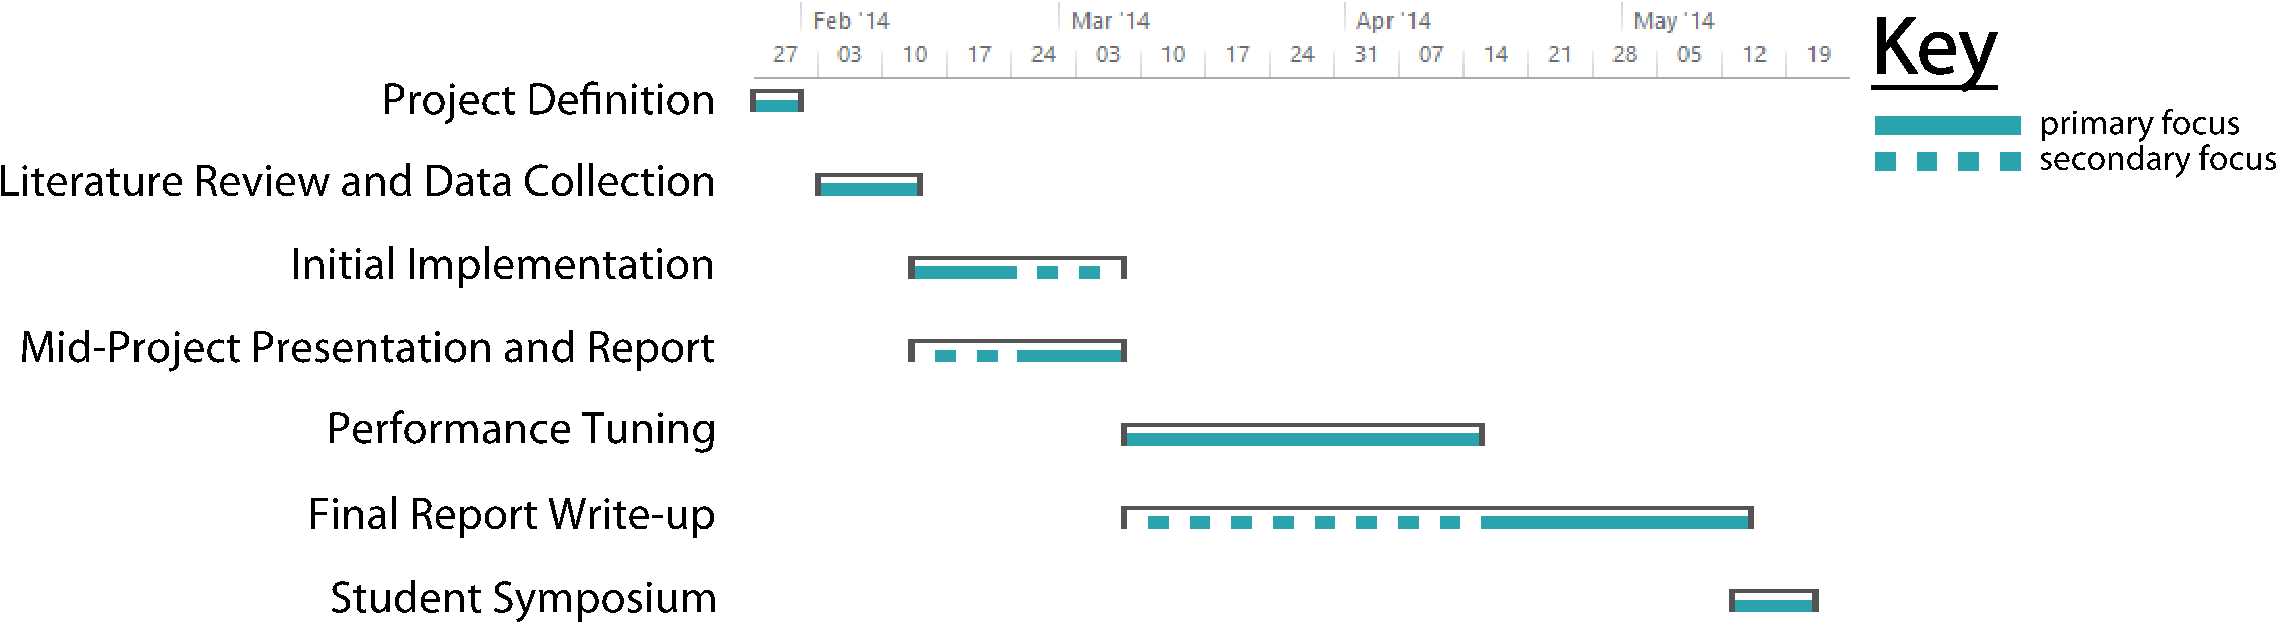
\includegraphics[scale=0.45]{figures/schedule/initial_project_schedule.pdf}
	}%
	\caption{Initial Project Schedule Created on 31/01/14}
	\label{fig:initial-schedule}
\end{figure}

\begin{figure}[h]
	\centering
	\makebox[\textwidth][c]{
		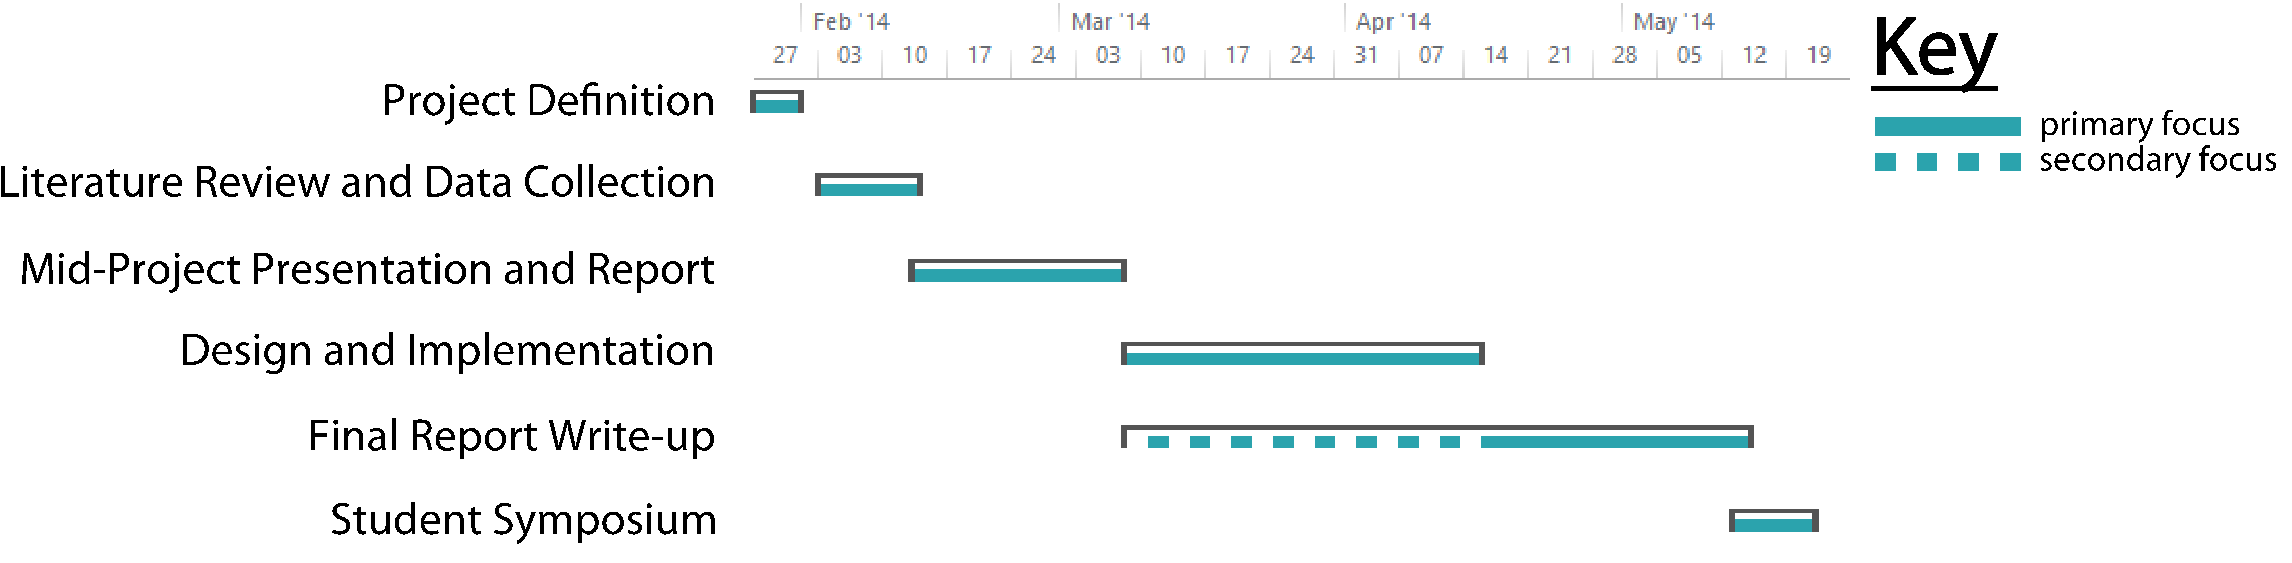
\includegraphics[scale=0.45]{figures/schedule/revised_project_schedule.pdf}
	}%
	\caption{Revised Project Schedule Created on 20/02/14}
	\label{fig:revised-schedule}
\end{figure}

\begin{figure}[h]
	\centering
	\makebox[\textwidth][c]{
		\includegraphics[scale=0.6]{figures/schedule/full-project-process.pdf}
	}%
	\caption{Flow Chart of Full Project Schedule}
	\label{fig:full-project-process}
\end{figure}

\begin{landscape}	
	\begin{figure}
		\centering
		\centerline{ 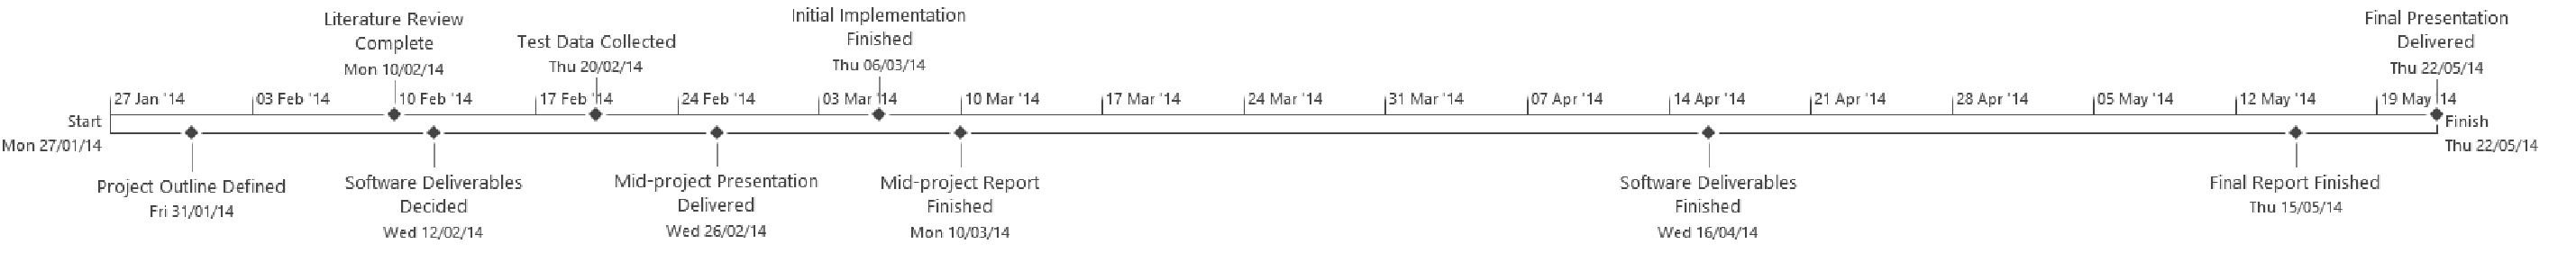
\includegraphics[scale=0.475]{figures/schedule/initial_schedule_timeline.pdf} }
		\caption{Initial Milestone Timeline Created on 20/02/14}
		\label{fig:initial-milestone-timeline}
	\end{figure}

	\begin{figure}
		\centering
		\centerline{ 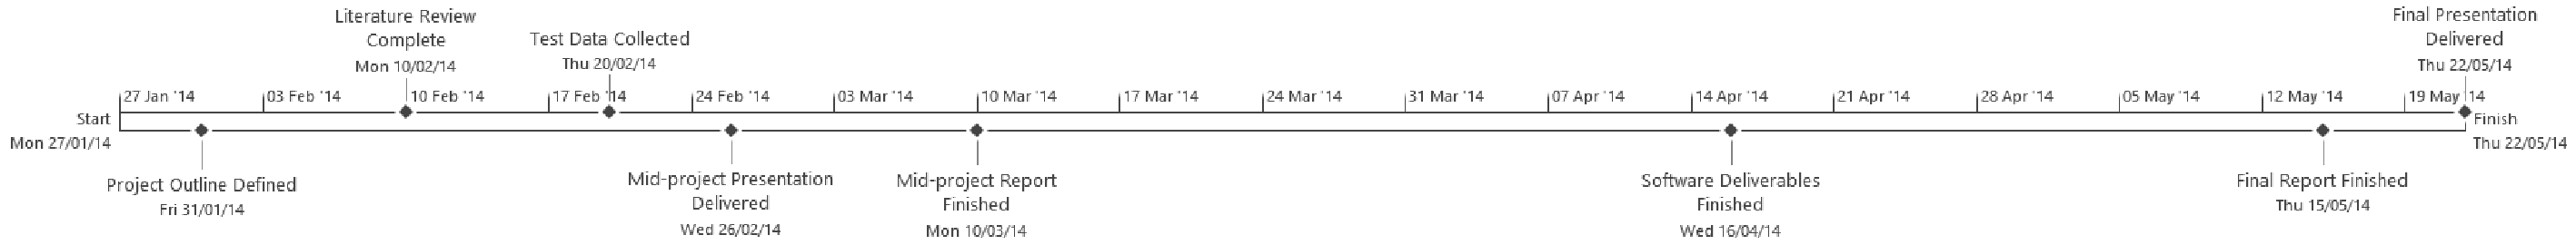
\includegraphics[scale=0.475]{figures/schedule/revised_schedule_timeline.pdf} }
		\caption{Revised Milestone Timeline Created on 20/02/14}
		\label{fig:revised-milestone-timeline}
	\end{figure}	
\end{landscape}




\begin{landscape}
	\section{Multi-dimensional Search Structures}

	TODO: intro

	\begin{table}[h]
		\centering
		\begin{tabular}{|p{2.8cm}|p{5cm}|p{5cm}|p{5cm}|p{2cm}|}
			\hline
			\textbf{Index Structure} &
			\textbf{Memory Overhead} &
			\textbf{Bucket Method?} &
			\textbf{High-Dimensional Data} &
			\textbf{Complexity} \\
			\hline
			Sequential Scan & Low & No (but since data is stored contiguously, there are minimal I/O operations due to sequential access) & Often better than other structures with high $d$ (but significantly poorer performance with low $d$) & Low \\		
			B${}^{+}$-Tree & Low & Yes & One-dimensional & Low \\
			R-Tree & Moderate & Yes & Poor for $d > 10$ \cite{pyramid-tree} & Moderate \\
			Quadtree & Low with uniformly distributed data, high for skewed data due to unnecessary nodes caused by splitting sparse regions of data space & No & Poor because it tries to use balanced splits \cite{pyramid-tree} & Low \\
			Pyramid Tree & Low & Yes (based on B${}^{+}$-tree) & Good & High \\
			PK-Tree & Moderate & No (but uses similar method to reduce I/O operations) & Good & High \\
			Skip Quadtree & Moderate & No & Untested & Moderate \\
			Quadtreap & Low & No & Untested & Moderate \\
			Splay Quadtree & Moderate & No & Untested & Moderate \\
			\hline
		\end{tabular}
		\caption{Comparison of Dynamic Multi-Dimensional Structures}
		\label{tab:comparison}
	\end{table}

	\null  % Empty line
	\nointerlineskip  % No skip for prev line
	\vfill
	\let\snewpage \newpage
	\let\newpage \relax
		\begin{figure}[H]
			\centering
			\includegraphics[scale=0.35]{figures/md_structure_taxonomy.png}
			\caption{Multi-dimensional Search Structure Taxonomy}
			\label{fig:structure-taxonomy}
		\end{figure}
	\let \newpage \snewpage
	\vfill 
	\break % page break

	\newpage

\end{landscape}




\section{Performance Timings}

TODO: intro

=ITERATION 1=
TODO: tables showing times for three operations w/ synthetic and clustered data (two tables)

=ITERATION 3=
TODO: tables showing times for three operations w/ synthetic and clustered data (two tables)




\section{Algorithms and Code Listings}

TODO: intro

\begin{algorithm}[H]
	\SetAlgoLined
	\SetKwInOut{Input}{input}\SetKwInOut{Output}{output}
	\SetKwFunction{hashPoint}{hashPoint} \SetKwFunction{hashFloat}{hashFloat}

 	\SetKwProg{funcHashPoint}{Algorithm}{}{}
  	\funcHashPoint{\hashPoint{$d, p$}} {
		\Input{$d$ = number of dimensions}
		\Input{$p_0, p_1, \dots, p_{d-1}$ = coordinates of point}
		\Output{$seed$ = integer representing hashed point}
		\Begin {
			$seed = 0$\;
			\For{$i = 0$ to $d - 1$} {
				$seed = seed \oplus \left(\hashFloat(p_i) + \texttt{0x9e3779b9} + (seed << 6) + (seed >> 2)\right)$
			}
			\KwRet{$seed$}
		}
	}

	\caption{Hashing Multi-Dimensional Point in Bucket Hash Table}
	\label{alg:point-hashing}
\end{algorithm}

\paragraph{\textbf{NOTE:}} \texttt{hashFloat} is a function which hashes an individual 32-bit floating point number and corresponds to the function \texttt{float\_hash\_impl2} in Listing \ref{lst:hash-float-function}.

\paragraph{} 

\begin{lstlisting}[label=lst:hash-float-function, caption=Code to Hash Single 32-bit Floating Point Value (Source code from file \texttt{boost/functional/hash/detail/hash\_float\_generic.hpp} in Boost Library 1.42.0)]
// Copyright 2005-2009 Daniel James.
// Distributed under the Boost Software License, Version 1.0. (See accompanying
// file LICENSE_1_0.txt or copy at http://www.boost.org/LICENSE_1_0.txt)

// A general purpose hash function for non-zero floating point values.

inline void hash_float_combine(std::size_t& seed, std::size_t value)
{
    seed ^= value + (seed<<6) + (seed>>2);
}

template <class T>
inline std::size_t float_hash_impl2(T v)
{
    boost::hash_detail::call_frexp<T> frexp;
    boost::hash_detail::call_ldexp<T> ldexp;

    int exp = 0;

    v = frexp(v, &exp);

    // A postive value is easier to hash, so combine the
    // sign with the exponent and use the absolute value.
    if(v < 0) {
        v = -v;
        exp += limits<T>::max_exponent -
            limits<T>::min_exponent;
    }

    // The result of frexp is always between 0.5 and 1, so its
    // top bit will always be 1. Subtract by 0.5 to remove that.
    v -= T(0.5);
    v = ldexp(v, limits<std::size_t>::digits + 1);
    std::size_t seed = static_cast<std::size_t>(v);
    v -= seed;

    // ceiling(digits(T) * log2(radix(T))/ digits(size_t)) - 1;
    std::size_t const length
        = (limits<T>::digits *
                boost::static_log2<limits<T>::radix>::value - 1)
        / limits<std::size_t>::digits;

    for(std::size_t i = 0; i != length; ++i)
    {
        v = ldexp(v, limits<std::size_t>::digits);
        std::size_t part = static_cast<std::size_t>(v);
        v -= part;
        hash_float_combine(seed, part);
    }

    hash_float_combine(seed, exp);

    return seed;
}
\end{lstlisting}

\end{document}
